\documentclass[11pt,a4paper]{article}

% ============================================================================
%  preambule.tex -- packages et reglages du rapport
%  (regenere : l'original avait ete ecrase par une image)
% ============================================================================

% --- Encodage et langue ---
\usepackage[utf8]{inputenc}
\usepackage[T1]{fontenc}
\usepackage[french]{babel}

% --- Mise en page ---
\usepackage{geometry}
\geometry{margin=2.5cm}
\usepackage{setspace}
\usepackage{parskip}

% --- Maths ---
\usepackage{amsmath}
\usepackage{amssymb}
\usepackage{bm}        % \bm{...} (symboles gras) utilise dans sec3 (Navier-Stokes)
\usepackage{siunitx}

% --- Figures et tableaux ---
\usepackage{graphicx}
% Cherche les images dans sections/images/ (puis images/ et le dossier courant)
\graphicspath{{sections/images/}{images/}{./}}
\usepackage{float}
\usepackage{subcaption}
\usepackage{caption}
\usepackage{booktabs}

% --- Liens cliquables ---
\usepackage{xcolor}
\usepackage{hyperref}
\hypersetup{
    colorlinks=true,
    linkcolor=blue,
    citecolor=blue,
    urlcolor=blue,
    pdftitle={Rapport d'avancement de stage -- IMFT},
    pdfauthor={Carl Bonjean Fraser}
}


\begin{document}

\begin{titlepage}
    \centering
    \begin{figure}[h!]
        \centering
        
\includegraphics[width=0.2\textwidth]{logo_imft.png}
    \end{figure}

    \vspace{1.5cm}

    {\large\bfseries ENSEEIHT -- Toulouse INP}\\[0.2cm]
    {\large Institut de Mécanique des Fluides de Toulouse (IMFT)}\\[1.5cm]

    \rule{\linewidth}{0.5mm} \\[0.4cm]
    {\huge\bfseries Effet de la turbulence sur la vitesse\\[0.2cm]
     d'ascension d'une bulle}\\[0.3cm]
    {\large\itshape Simulation numérique directe (Basilisk) d'une bulle
     en turbulence homogène isotrope}\\[0.3cm]
    \rule{\linewidth}{0.5mm} \\[2cm]

    \begin{minipage}{0.45\textwidth}
        \begin{flushleft} \large
            \emph{Auteur :}\\
            \textbf{Carl Bonjean Fraser}\\
            \small Étudiant Ingénieur (M1 / 2A MFEE)
        \end{flushleft}
    \end{minipage}
    ~
    \begin{minipage}{0.45\textwidth}
        \begin{flushright} \large
            \emph{Tuteurs de stage :}\\
            \textbf{LEGENDRE Dominique}\\
            \textbf{ZAMANSKY Rémi}
        \end{flushright}
    \end{minipage}

    \vfill
    {\large Rapport de stage}\\[0.2cm]
    {\large Année Universitaire 2025-2026 \quad--\quad Juin -- Juillet 2026}
\end{titlepage}

\newpage
\begin{abstract}
\noindent
On étudie par simulation numérique (solveur \texttt{Basilisk}, méthode
Volume-Of-Fluid, maillage octree adaptatif) l'ascension d'une bulle de gaz unique
($\rho_l/\rho_g = 850$, nombre de Bond $Bo=1$, nombre de Galilée $Ga=70$) dans une
turbulence homogène isotrope en boite triplement périodique. Nous cherchons a savoir 
si la turbulence ambiante accélère ou ralentit la remontée d'une bulle. En balayant
l'intensité turbulente $\beta = u'/u_\infty$, on montre que la turbulence
\textbf{ralentissent} systématiquement la remontée, de $-3\,\%$ à $\beta=0{,}05$ jusqu'à
$-72\,\%$ à $\beta=0{,}65$, en accord sans ajustement avec la courbe de référence de la
littérature. Une mesure directe du champ de vitesse vu par la bulle attribue ce
ralentissement à la \textbf{traînée non linéaire} plutôt qu'à un échantillonnage
préférentiel.
\end{abstract}

\newpage
\tableofcontents
\newpage

\section{Introduction}

La remontée d'une bulle de gaz dans un liquide au repos est l'un des problèmes les
plus anciens de la mécanique des fluides diphasiques. Nous etudions le cas d'une bulle 
remontant dans un écoulement porteur \emph{turbulent}. Les écoulements à bulles
turbulents interviennent dans un grand nombre de configurations naturelles et
industrielles : colonnes à bulles et réacteurs chimiques (aération, fermentation,
procédés d'oxydation), génie des procédés pétroliers, mais aussi processus
environnementaux à grande échelle comme les échanges gazeux à l'interface
océan-atmosphère sous l'effet du déferlement des vagues. Dans toutes ces
situations, la turbulence ambiante modifie la vitesse à laquelle le gaz remonte, 
et donc les temps de séjour, les taux de transfert de masse et, in fine, le rendement
des procédés concernés.

La question posée dans ce travail est simple à énoncer et difficile à trancher :
\emph{la turbulence ambiante accélère-t-elle ou ralentit-elle la vitesse
d'ascension d'une bulle, par rapport à sa vitesse terminale en liquide au repos ?}
Deux intuitions contradictoires coexistent dans la littérature. D'une part, la
turbulence pourrait favoriser la remontée en réduisant transitoirement la traînée
(par analogie avec la réduction de traînée observée sur des sphères solides en
écoulement turbulent) ou en permettant à la bulle d'exploiter des structures
tourbillonnaires porteuses. D'autre part, elle pourrait au contraire freiner la
bulle : en la faisant dévier de sa trajectoire rectiligne, en la faisant
échantillonner préférentiellement des zones de fluide descendant, ou en augmentant
sa traînée moyenne du fait de la non-linéarité de la loi de traînée vis-à-vis des
fluctuations de vitesse relative. Trancher entre ces scénarios est rendu difficile
par le couplage intrinsèque entre la bulle et la turbulence qui l'entoure : la
bulle déforme et perturbe localement l'écoulement porteur, son sillage instationnaire
interagit avec les structures turbulentes incidentes, et sa trajectoire peut devenir
oblique ou instable même en l'absence de toute turbulence dès lors que le nombre de
Galilée dépasse un seuil critique. Isoler l'effet net de la turbulence sur la
vitesse de remontée exige donc une simulation où les autres
paramètres du problème (rapports de densité et de viscosité, tension superficielle,
taille de bulle) sont maîtrisés et maintenus fixes pendant que l'intensité
turbulente varie seule.

\subsection{État de l'art}

Le ralentissement de la remontée d'une bulle par la turbulence ambiante est un
problème débattu de longue date. Sur le plan expérimental, Poorte \& Biesheuvel
\cite{poorte2002} ont mesuré, dans une turbulence de grille quasi homogène et
isotrope, une réduction de la vitesse moyenne d'ascension pouvant atteindre
environ $-35\,\%$ par rapport à la valeur en liquide au repos, établissant
empiriquement que l'effet net de la turbulence est bien un ralentissement et non
une accélération. Sur le plan théorique, Spelt \& Biesheuvel \cite{spelt1997} ont
proposé, dans la limite d'une turbulence de faible intensité, une loi de
correction quadratique de la forme $1 - c\,\beta^2$, où $\beta = u'/u_\infty$ est
le rapport entre la fluctuation de vitesse turbulente $u'$ et la vitesse
terminale en milieu quiescent $u_\infty$ : la réduction relative de vitesse croît
comme le carré de l'intensité turbulente relative au voisinage de $\beta = 0$.
À l'opposé, dans le régime de turbulence forte, Ruth \emph{et al.}
\cite{ruth2021} ont montré que la réduction de vitesse suit asymptotiquement une
loi en $0.37/\mathrm{Fr}'$, où $\mathrm{Fr}' = u'/\sqrt{gD}$ est un nombre de
Froude turbulent construit sur la fluctuation de vitesse et le diamètre de bulle
$D$ : au-delà d'un certain régime, c'est la dynamique de grand nombre de Froude
turbulent, et non plus l'intensité turbulente relative $\beta$, qui contrôle
directement la réduction de vitesse.

Ces deux comportements ont été réunis en une courbe  par Liu, Farsoiya, Perrard \& Deike \cite{liu2024}, au moyen de simulations
numériques directes réalisées avec le même solveur (Basilisk) et sur le même type
de configuration (une bulle unique en turbulence homogène isotrope triplement
périodique) que celle utilisée dans le présent travail. Cette étude sera la
référence  du présent stage : elle relie le régime petite
perturbation ($1-c\beta^2$) au régime grand nombre de Froude turbulent
($0.37/\mathrm{Fr}'$), et surtout elle attribue explicitement le mécanisme du
ralentissement à la \emph{traînée non linéaire} : la loi de traînée $C_D(Re)$
n'étant pas linéaire en la vitesse relative, des fluctuations symétriques de
cette vitesse relative induites par la turbulence produisent, en moyenne, une
traînée plus grande que celle évaluée à la vitesse moyenne, d'où un
ralentissement systématique. Ce mécanisme est explicitement distingué de
l'\emph{échantillonnage préférentiel} (biais statistique par lequel une
bulle plus légère que le fluide environnant a tendance à être capturée par les
zones de vorticité et de fluide descendant). Ce mécanisme, selon Liu \emph{et
al.}, domine plutôt pour des bulles de taille inférieure ou de l'ordre de
l'échelle de Kolmogorov (nombre de Stokes $\mathrm{St} \sim 1$), alors que la
traînée non linéaire domine pour des bulles de taille supérieure à cette échelle
($\mathrm{St} \gg 1$), configuration qui est celle du présent travail.

Le paramètre de contrôle central de ce problème a été mis en évidence par la
revue récente de Legendre \& Zenit \cite{legendre2025} (\emph{Reviews of Modern
Physics}) : c'est le rapport $\beta = u'/u_\infty$ entre la fluctuation de
vitesse turbulente et la vitesse terminale en milieu au repos qui organise
l'ensemble des résultats de la littérature. D'autres travaux de simulation numérique
directe éclairent des aspects connexes du problème : Loisy \& Naso
\cite{loisy2017} ont étudié le cas d'une grosse bulle flottante en turbulence
homogène isotrope, dans un régime de tailles comparable à celui considéré ici ;
Cano-Lozano \& Magnaudet \cite{canolozano2016} ont caractérisé l'instabilité de
trajectoire d'une bulle isolée en liquide au repos, montrant qu'elle devient
oblique ou instationnaire au-delà d'un nombre de Galilée critique
$\mathrm{Ga}_c \approx 44$ ; enfin Rivière \emph{et al.} \cite{riviere2021} ont
caractérisé la fragmentation d'une bulle en turbulence, avec un seuil critique en
nombre de Weber turbulent $\mathrm{We}_c \approx 3$, qui borne le domaine des
intensités turbulentes explorables sans rupture de la bulle.

De cette littérature se dégagent trois éléments structurants pour la présente
étude. Premièrement, le paramètre de contrôle pertinent est $\beta = u'/u_\infty$. Deuxièmement, la réduction relative de vitesse
$u_{\infty,\mathrm{turb}}/u_\infty$ suit deux régimes asymptotiques distincts : une
loi quadratique $1-c\beta^2$ à petit $\beta$, puis une loi en $1/\mathrm{Fr}'$ à
grand nombre de Froude turbulent, les deux étant reliées par la courbe de référence
de Liu \emph{et al.} \cite{liu2024}. Troisièmement, le mécanisme physique
responsable du ralentissement fait débat entre échantillonnage préférentiel et
traînée non linéaire, les deux mécanismes n'étant pas mutuellement exclusifs mais
opérant préférentiellement dans des régimes de taille de bulle différents
(sous-Kolmogorov contre super-Kolmogorov).

%%% Ajouter ici une figure de la courbe maitresse de liu et al

\subsection{Objectifs et plan du rapport}

L'objectif de ce travail est de quantifier, par simulation numérique, la
réduction relative de la vitesse d'ascension $u_{\infty,\mathrm{turb}}/u_\infty$
d'une bulle unique en fonction de l'intensité turbulente relative $\beta$, à
nombre de Bond $\mathrm{Bo}=1$ et nombre de Galilée $\mathrm{Ga}=70$ fixés (donc
au-delà du seuil d'instabilité de trajectoire $\mathrm{Ga}_c\approx44$ identifié
par Cano-Lozano \& Magnaudet \cite{canolozano2016}), et d'identifier lequel des
deux mécanismes candidats 1. échantillonnage préférentiel ou 2. traînée non linéaire domine dans le régime de taille de bulle considéré, en faisant la confrontation aux résultats de Liu, Farsoiya, Perrard \& Deike
\cite{liu2024}.

La suite du rapport est organisée comme suit. La section~2 pose le cadre physique
et adimensionnel du problème (Vaschy-Buckingham, définition de
$\beta$ et de $\mathrm{Fr}'$). La section~3 décrit les méthodes numériques :
solveur Basilisk, méthode VOF conservant la quantité de mouvement, raffinement de
maillage adaptatif par octree, protocole en deux étapes précurseur turbulent puis
injection de la bulle. La section~4 présente la validation du modèle numérique
(convergence en maillage, courants parasites, biais liés à la périodicité du
domaine). La section~5 présente les résultats : effet mesuré de la turbulence sur
la vitesse d'ascension en fonction de $\beta$. La section~6 discute le mécanisme
physique du ralentissement observé. La section~7 conclut et dégage les
perspectives de ce travail.

\section{Cadre physique et adimensionnel}
\label{sec:cadre}

Cette section pose les grandeurs physiques du problème ainsi que les nombres sans dimension qui le décrivent. Elle
établit, par une analyse de Buckingham, que ce problème comporte
trois nombres sans dimension indépendants, ce qui fixe la
structure de toute la campagne de simulations présentée dans les sections
suivantes.

\subsection{Grandeurs physiques}
\label{sec:cadre:grandeurs}

Le système est diphasique : un liquide (indice $l$) porte une bulle de gaz
(indice $g$), la bulle étant la phase légère repérée par la fraction
volumique $f<0{,}5$ (convention $f=1$ dans le liquide, $f=0$ dans le gaz,
détaillée en section Méthodes). Chaque phase est caractérisée par sa masse
volumique $\rho$ et sa viscosité dynamique $\mu$ (ou cinématique
$\nu=\mu/\rho$), l'interface qui les sépare par une tension superficielle
$\sigma$, et le champ de pesanteur uniforme $g$ ferme le système.

Le moteur de l'ascension est la \textbf{poussée d'Archimède}, proportionnelle
à l'écart de densité $\Delta\rho = \rho_l - \rho_g$ et à $g$. Pour que cette
poussée soit correctement représentée dans un domaine \emph{périodique}, cette force issue la gravité est formulée comme une force volumique périodique, de moyenne nulle sur le
domaine :
\begin{equation}
    \rho\,\mathbf{a} = (\rho - \rho_m)\,\mathbf{g},
    \qquad \rho_m = \langle \rho \rangle_{\text{domaine}},
    \label{eq:archimede}
\end{equation}
où $\rho_m$ est la densité moyenne du domaine.

Les rapports de propriétés entre phases sont fixés une fois pour toutes sur
l'ensemble de l'étude, dans le régime d'une bulle de gaz légère et peu visqueuse en
milieu liquide :
\begin{equation}
    \frac{\rho_l}{\rho_g} = 850, \qquad \frac{\mu_l}{\mu_g} = 100.
    \label{eq:rapports}
\end{equation}
Le rapport de densité est celui d'un couple air/eau, également retenu par les simulations de
référence~\cite{riviere2021,liu2024}~; le rapport de viscosité est ici plus élevé que
la valeur $\mu_l/\mu_g=25$ de ces études, sans incidence sur la dynamique aux nombres
de Reynolds de bulle considérés, la phase gazeuse restant dynamiquement passive.
Le diamètre de bulle
$D$ (diamètre équivalent d'une sphère de même volume) est la longueur de
référence du problème ; la géométrie du domaine (taille $L_0$, triplement
périodique) est elle aussi fixée.

\subsection{Nombres sans dimension}
\label{sec:cadre:nombres}

Cinq groupements sans dimension organisent la discussion physique du
problème : trois nombres microscopiques classiques de la dynamique d'une
bulle isolée (Bond, Galilée, Reynolds de bulle) et deux nombres qui
caractérisent l'agitation turbulente extérieure vue par la bulle (Weber
turbulent, Reynolds turbulent), le tout relié par un paramètre central,
$\beta$, propre au cadre de couplage bulle-turbulence.

\paragraph{Nombre de Bond.} Il compare la flottabilité, motrice de la
déformation, à la tension superficielle, qui s'y oppose :
\begin{equation}
    Bo = \frac{\Delta\rho\, g\, D^2}{\sigma}.
    \label{eq:bond}
\end{equation}
Il est imposé à $Bo=1$ sur l'ensemble de l'étude (bulle modérément
déformable).

\paragraph{Nombre de Galilée.} Il compare les forces de flottabilité aux
forces visqueuses et gouverne, à $Bo$ fixé, le régime de sillage et de
trajectoire d'une bulle isolée en fluide au repos :
\begin{equation}
    Ga = \frac{\sqrt{g D^3}}{\nu}.
    \label{eq:galilee}
\end{equation}
Il vaut $Ga=70$ dans toute la campagne. Sur le diagramme des régimes
$(Ga,Bo)$ établi par \cite{canolozano2016}, ce couple se situe au-delà du
seuil de stabilité de la trajectoire rectiligne, $Ga_c\simeq44$ à $Bo=1$ : on s'attend alors a
une trajectoire \textbf{oblique}.

\paragraph{Nombre de Reynolds de bulle.} Une fois la vitesse terminale
$u_\infty$ mesurée, il quantifie a posteriori le régime inertiel de
l'écoulement autour de la bulle :
\begin{equation}
    Re_b = \frac{u_\infty D}{\nu}.
    \label{eq:reb}
\end{equation}
La référence laminaire de cette étude (bulle isolée en liquide au repos)
donne $Re_b \approx 108$.

\paragraph{Nombre de Weber turbulent.} Il compare l'agitation turbulente
ambiante à
la tension superficielle, et gouverne la possibilité de rupture de la
bulle :
\begin{equation}
    We_t = \frac{\rho_l\, u'^2\, D}{\sigma},
    \label{eq:wet}
\end{equation}
où $u'$ est la vitesse fluctuante du liquide loin de la bulle. Sa
définition et le seuil de rupture associé $We_{tC}=\mathcal{O}(1)$ suivent la
revue de \cite{legendre2025} ; l'ordre de grandeur $We_c\approx3$ est
également rapporté par \cite{riviere2021}.

\paragraph{Nombre de Reynolds turbulent.} Il caractérise, indépendamment de
l'intensité $u'$, l'étendue de la cascade inertielle de la turbulence
porteuse, via l'échelle de Taylor $\lambda$ :
\begin{equation}
    Re_\lambda = \frac{u'\,\lambda}{\nu}.
    \label{eq:relambda}
\end{equation}

\paragraph{Froude turbulent et paramètre $\beta$.} Deux
grandeurs de référence sont possibles : la vitesse d'échelle de flottabilité
$\sqrt{gD}$, donnant le \textbf{Froude turbulent}
\begin{equation}
    Fr' = \frac{u'}{\sqrt{gD}},
    \label{eq:frprime}
\end{equation}
et la vitesse terminale \emph{mesurée} en liquide au repos $u_\infty$,
donnant le paramètre
\begin{equation}
    \beta = \frac{u'}{u_\infty},
    \label{eq:beta}
\end{equation}
identifié par \cite{legendre2025} comme un paramètre de contrôle du
couplage bulle-turbulence dans la littérature du domaine. Les deux sont
reliés, une fois $u_\infty$ connu, par le rapport (constant pour cette étude)
$\sqrt{gD}/u_\infty$, soit numériquement
\begin{equation}
    Fr' = 1{,}53\,\beta.
    \label{eq:fr_beta}
\end{equation}
Les deux paramètres ($\beta$ et $Fr'$) seront utilisés en parallèle dans la suite du rapport.

\subsection{Analyse dimensionnelle : trois groupes indépendants}
\label{sec:cadre:buckingham}

Une fois les rapports de densité et de viscosité \eqref{eq:rapports} et la
géométrie fixés, le problème --- une bulle de diamètre $D$ dans un liquide de
masse volumique $\rho_l$ et de viscosité cinématique $\nu$, soumise à la
pesanteur $g$, à une tension superficielle $\sigma$, et à une turbulence
extérieure de dissipation $\varepsilon$ --- fait intervenir six grandeurs
dimensionnelles : $g,\ \sigma,\ \nu,\ \varepsilon,\ \rho_l,\ D$. Ces six
grandeurs s'expriment avec trois dimensions fondamentales indépendantes
($M$, $L$, $T$). Le théorème de Vaschy--Buckingham donne donc
\begin{equation}
    6 \text{ grandeurs} - 3 \text{ dimensions} = 3 \text{ groupes sans dimension indépendants}.
    \label{eq:buckingham}
\end{equation}
On les choisit comme $Bo$, $We_t$ et $Re_\lambda$. Le quatrième
nombre usuel de la dynamique des bulles, le Galilée $Ga$ (ou, de façon
équivalente, le nombre de Morton $Mo = Bo^3/Ga^4$), ne sont pas libres et dérivent du choix des autres paramètres.

\subsection{Concepts numériques}
\label{sec:cadre:numerique}

La résolution du problème diphasique repose sur trois choix numériques dont
le détail (schémas, critères, implémentation) est développé en section
Méthodes ; ils sont seulement introduits ici pour situer le vocabulaire
utilisé dans la suite.

\begin{itemize}
\item \textbf{Volume-Of-Fluid (VOF).} On repère l'interface liquide/gaz avec la fraction volumique $f$ ($f=1$ dans le liquide, $f=0$ dans le gaz). Son advection préserve la masse de chaque phase. On utilise une formulation qui conserve aussi la quantité de mouvement, ce qui est crucial vu le fort écart de densité ($\rho_l/\rho_g=850$) de l'étude.
    \item \textbf{Maillage adaptatif octree.} Le domaine, discrétisé en
    arbre octree, est raffiné localement où l'erreur d'ondelette dépasse un
    seuil, sur les champs $\{f, |\boldsymbol{\omega}|\}$ (interface et
    vorticité) : l'interface de la bulle et son sillage turbulent sont
    résolus finement, le reste du domaine reste grossier.
    \item \textbf{Unités code.} L'ensemble des simulations est mené en
    unités adimensionnées par la masse volumique du liquide ($\rho_l=1$),
    l'intensité de la pesanteur ($g$ pris comme échelle d'accélération) et
    le rayon initial de la bulle $R_0$ comme longueur de référence. Les
    nombres sans dimension de \S\ref{sec:cadre:nombres} sont donc directement
    lisibles sur les grandeurs codées, sans conversion.
\end{itemize}

\section{Méthodes numériques}
\label{sec:methodes}

\subsection{Solveur}
\label{subsec:solveur}

Nous utilisons le code \textsc{Basilisk}, un solveur d'équations aux dérivées partielles sur maillage octree adaptatif. Le code source écrit en C étendu (boucles \texttt{foreach}, opérateurs différentiels, événements temporels) est traduit en C standard par le précompilateur \texttt{qcc}, puis compilé avec \texttt{mpicc} pour l'exécution parallèle. Les simulations tournent sous MPI sur le cluster CALMIP (projet Kairos, IMFT). Ce solveur a déjà fait ses preuves pour les écoulements diphasiques turbulents à interface déformable, notamment sur la déformation~\cite{perrard2021} et la fragmentation~\cite{riviere2021} de bulles, l'ascension d'une bulle en THI~\cite{liu2024} ou la fragmentation de gouttes visqueuses~\cite{farsoiya2023}. Nous reprenons ici la même méthodologie.

Le système diphasique fluide/gaz est incalculable sous forme séparée sans approximations lourdes. Nous le résolvons donc avec une formulation « un fluide ». Un seul champ de vitesse $\mathbf{u}$ et un seul champ de pression $p$ décrivent tout le domaine :
\begin{align}
    \rho\left(\partial_t \mathbf{u} + \mathbf{u}\cdot\nabla\mathbf{u}\right)
        &= -\nabla p + \nabla\cdot\left(2\mu\,\mathbf{D}\right)
           + \sigma\,\kappa\,\delta_s\,\mathbf{n} + \rho\,\mathbf{a}, \\
    \nabla\cdot\mathbf{u} &= 0,
\end{align}
avec $\mathbf{D}$ le tenseur des taux de déformation, $\sigma\kappa\delta_s\mathbf{n}$ la force de tension superficielle localisée à l'interface (courbure $\kappa$, normale $\mathbf{n}$) et $\mathbf{a}$ un terme d'accélération volumique (gravité et forçage turbulent). La densité $\rho$ et la viscosité $\mu$ varient brutalement à la traversée de l'interface. Elles dépendent de la fraction volumique $f$, suivie par la méthode \textbf{Volume-Of-Fluid} (VOF) :
\begin{equation}
    \partial_t f + \nabla\cdot(f\,\mathbf{u}) = 0, \qquad
    \rho = f\,\rho_1 + (1-f)\,\rho_2, \qquad
    \mu = f\,\mu_1 + (1-f)\,\mu_2,
\end{equation}
où $f=1$ correspond au liquide et $f=0$ au gaz. L'interface est reconstruite géométriquement à chaque pas de temps par un plan coupe-maille (reconstruction linéaire par morceaux). Cela évite de l'étaler numériquement et maintient son épaisseur sur une à deux mailles au cours du temps.

\paragraph{Advection conservant la quantité de mouvement.} Notre rapport de densité liquide/gaz est fort ($\rho_1/\rho_2 = 850$). Si l'on transporte $f$ par de la géométrie mais qu'on advecte la vitesse $\mathbf{u}$ séparément avec un schéma classique, on crée un décalage entre le flux de masse et le flux de quantité de mouvement. Cela produit des courants parasites et de l'instabilité près de la bulle. Pour éviter ce problème, Basilisk utilise un schéma VOF qui conserve la quantité de mouvement \cite{popinet2009} : le même flux géométrique qui déplace $f$ sert aussi à transporter $\rho\mathbf{u}$. C'est indispensable pour stabiliser nos calculs.

\paragraph{Tension superficielle.} Nous modélisons la tension superficielle via une force de surface continue (CSF) sous forme équilibrée (\emph{balanced-force}). Cette formulation annule exactement le gradient de pression et le saut de Laplace à l'équilibre au niveau discret, ce qui bloque l'apparition de courants parasites sur une interface peu déformée. La courbure locale est calculée par la méthode des fonctions de hauteur.

\paragraph{Maillage adaptatif.} La discrétisation repose sur une grille \textbf{octree}, raffinée localement grâce à la fonction \texttt{adapt\_wavelet}. À chaque pas de temps, l'algorithme évalue l'erreur d'estimation en ondelettes sur des champs cibles (fraction volumique, vorticité). Si l'erreur dépasse un seuil donné, la maille est divisée ; si elle repasse en dessous d'une fraction de ce seuil, la maille est fusionnée. Cet effet d'hystérésis évite que le maillage ne clignote d'un pas de temps à l'autre. La résolution se concentre donc d'elle-même sur l'interface et les tourbillons, tout en restant grossière dans le reste du domaine. Les champs et les seuils utilisés changent selon la phase de simulation et sont détaillés en section \ref{subsec:forcage} et \ref{subsec:protocole}.

Le domaine de calcul est un cube triplement périodique de côté $L_0 = 120$ (unités code). Nous y plaçons une unique bulle sphérique de rayon $R_0 = 8$ ($D=16$, soit un rapport $L_0/D = 7{,}5$) au centre. Pour le parallélisme MPI, Basilisk découpe l'arbre octree le long d'une courbe de remplissage de l'espace et rééquilibre la charge entre les processeurs au fil du calcul.

\subsection{Génération de la turbulence : forçage linéaire contrôlé}
\label{subsec:forcage}

Nous entretenons la turbulence homogène isotrope (THI) par un forçage en espace physique, proportionnel à la vitesse locale du liquide. Proposé par \cite{rosales2005} et disponible dans l'exemple \texttt{isotropic.c} de Basilisk \cite{basilisk_isotropic}, ce principe produit une THI de qualité comparable à celle d'un code spectral. Nous utilisons ici la variante à énergie contrôlée de \cite{bassenne2016} : au lieu d'imposer une force fixe, l'algorithme vise directement une énergie cinétique cible (\texttt{KE\_TARGET}). À chaque pas de temps, nous appliquons une accélération :
\begin{equation}
    \mathbf{a}_{\text{forçage}} = A\,\left(\mathbf{u} - \overline{\mathbf{u}}\right),
    \qquad
    A = \frac{\varepsilon + \dfrac{\texttt{KE\_TARGET} - k}{\tau}}{2\,k},
    \qquad \tau = \frac{k}{\varepsilon},
    \label{eq:forcage}
\end{equation}
où $k$ et $\varepsilon$ sont l'énergie cinétique et sa dissipation, mesurées sur le champ au pas précédent (ce qui reste négligeable devant le temps de retournement). La puissance injectée ($2Ak$) équilibre la dissipation à l'état stationnaire. L'intensité turbulente devient alors une simple variable d'entrée fixée par l'utilisateur, ce qui nous permet de la balayer facilement au cours de l'étude.

\paragraph{Condition initiale.} Un simple mode ABC (Arnold--Beltrami--Childress) reste une solution stationnaire des équations d'Euler : le terme advectif se réduit à un gradient de pression. Injecter de l'énergie sur un tel champ ne fait qu'amplifier une structure figée, sans jamais lancer la cascade turbulente. Nous démarrons donc avec une superposition de trois modes ABC aux nombres d'onde $k=1,2,3$ (pondérés par $w_k = \{1;\,0{,}7;\,0{,}5\}$ et remis à l'échelle de l'énergie cible), avec $10\,\%$ de bruit blanc. La non-linéarité casse la symétrie et déclenche la cascade en quelques temps de retournement, ce que l'on observe très bien sur la montée du taux de dissipation $\varepsilon$.

\paragraph{Adaptation de maillage.} Durant la phase précurseur monophasique, nous gardons un maillage uniforme. Adaptativement raffiner un écoulement transitoire n'a pas d'intérêt et risque de couper des structures en formation. Une fois l'état stationnaire atteint, nous activons l'adaptation uniquement sur la vorticité $|\bm{\omega}|$. Le seuil d'erreur en ondelettes est réglé en fonction de la vorticité moyenne du champ, ce qui adapte automatiquement la grille peu importe la valeur de \texttt{KE\_TARGET}.

\subsection{Protocole précurseur $\to$ injection}
\label{subsec:protocole}

Nous n'injectons pas la bulle dès le début de la simulation. Le protocole se déroule en deux étapes, selon la méthode développée par le groupe de Deike pour l'étude des bulles en THI \cite{riviere2021,liu2024} et basée sur les exemples \texttt{bubble.c} \cite{basilisk_bubble} et \texttt{turbulent\_bubble.c} \cite{basilisk_turbbubble} de Basilisk :

\begin{enumerate}
    \item \textbf{Précurseur (phase monophasique, $f=1$ partout) :} nous laissons la turbulence se développer à partir du champ multi-modes initial. Une fois le régime stationnaire atteint à l'énergie \texttt{KE\_TARGET} voulue, nous sauvegardons l'état complet du calcul (vitesse et maillage) dans un fichier de reprise (\emph{dump}).
    
    \item \textbf{Injection de la bulle (phase diphasique) :} nous repartons du champ précurseur. Avant d'initialiser la bulle, nous raffinons le maillage dans la zone d'injection pour bien la résoudre dès le premier pas de temps. Nous imposerons ensuite la fraction volumique d'une sphère de rayon $R_0$ au centre du domaine, puis nous activons les équations diphasiques (tension superficielle, gravité, forçage) pour observer la remontée et la déformation.
\end{enumerate}

Cette approche garantit que la bulle entre dans une turbulence déjà mature, dont les grandeurs clés ($k$, $\varepsilon$, $Re_\lambda$, $\eta$) sont parfaitement mesurées. On évite ainsi de polluer les mesures avec le régime transitoire de création de la turbulence. De plus, la gravité n'impactant pas le champ monophasique, nous pouvons réutiliser un même précurseur pour tester plusieurs jeux de paramètres (tension superficielle, flottabilité) sans réinitialiser la turbulence à chaque fois.

\subsection{Gravité compatible avec la périodicité}
\label{subsec:gravite}

Notre domaine étant triplement périodique, nous ne pouvons pas utiliser la formulation usuelle en gravité réduite. Cette dernière exprime la poussée d'Archimède via un potentiel $\phi = [\rho]\,\mathbf{g}\cdot(\mathbf{x}-\mathbf{Z})$, linéaire selon $z$ et donc incompatible avec la périodicité aux frontières du domaine ($z=0 \leftrightarrow z=L_0$). Appliquer ce potentiel sur une frontière périodique génère une force parasite dès que la bulle la traverse (nous le montrons en détail dans la section de validation).

Pour contourner ce problème, nous définissons la gravité comme une force volumique périodique en retranchant la densité moyenne du domaine $\rho_m = \langle\rho\rangle$ :
\begin{equation}
    \rho\,\mathbf{a} = \left(\rho - \rho_m\right)\mathbf{g}
    \qquad\Longleftrightarrow\qquad
    a_z = -g\left(1 - \frac{\rho_m}{\rho}\right).
    \label{eq:force_perio}
\end{equation}

Cette approche offre trois avantages directs :
\begin{enumerate}
    \item La force dépend uniquement de la densité localement périodique $\rho(\mathbf{x})$. La bulle peut donc traverser les limites du domaine sans créer d'artefact.
    \item Sa moyenne volumique est nulle ($\int_V (\rho-\rho_m)\,\mathbf{g}\,\mathrm{d}V = 0$). Elle n'injecte aucune quantité de mouvement globale dans la boîte, ce qui est obligatoire en périodique.
    \item En phase monophasique ($\rho=\rho_m$), le terme $a_z$ s'annule exactement. La gravité n'impacte pas le précurseur turbulent, ce qui nous permet de réutiliser le même champ monophasique pour varier Bond et Weber.
\end{enumerate}

En contrepartie, cette formulation perd le caractère \emph{well-balanced} : la bulle subit une accélération apparente en $g\,\rho_m/\rho_2$, équilibrée au niveau du solveur de pression plutôt qu'au niveau discret exact. C'est le compromis nécessaire pour conserver la périodicité. Nous validons ce choix sur un cas test dédié dans la section suivante.

\subsection{Repère mobile}
\label{subsec:repere}

Lorsque la bulle traverse plusieurs fois le domaine périodique, les erreurs d'advection VOF s'accumulent à chaque franchissement de mailles. À terme, cette dérive altère le volume de la bulle et biaise sa vitesse d'ascension.

Pour résoudre ce problème, nous exploitons l'invariance galiléenne : retrancher une vitesse uniforme au champ conserve la dynamique de l'écoulement relatif. Le solveur suit donc la bulle en la centrant dans le domaine, la vitesse du repère s'ajustant avec un temps de relaxation $\tau_f$ :
\begin{equation}
    u_z \;\leftarrow\; u_z - \delta, \qquad
    \delta = \frac{\mathrm{d}t}{\tau_f}\,\overline{u_z}\big|_{\text{gaz}},
    \qquad
    U_f \;\leftarrow\; U_f + \delta,
    \label{eq:repere_mobile}
\end{equation}
où $\overline{u_z}|_{\text{gaz}}$ est la vitesse verticale moyenne du gaz et $U_f$ la vitesse cumulée du repère. La position au laboratoire s'obtient par intégration ($z_{\text{lab}}(t) = \int U_f\,\mathrm{d}t$), et la vitesse terminale $u_\infty$ correspond à la valeur stabilisée de $U_f$ (enregistrée dans \texttt{frame.dat}).

Le choix d'une relaxation progressive sur $\tau_f$ (de l'ordre de l'unité de temps) évite les accélérations d'entraînement brutales, sources de forces d'inertie parasites. Une fois le régime établi atteint, $U_f$ devient constant, le repère redevient strictement galiléen et la correction $\delta$ s'annule.

Nous contrôlons ce changement de repère via un suivi de la quantité de mouvement globale dans le repère du laboratoire (\texttt{momentum.dat}). Reconstruite avec la vitesse $U_f$, cette quantité de mouvement doit rester nulle sur tous les axes. Cela garantit qu'aucune force numérique non physique ne vient fausser le bilan global.

\subsection{Mesures d'ensemble}
\label{subsec:ensemble}

À nombre de Bond fixé, nous balayons l'intensité turbulente en faisant varier \texttt{KE\_TARGET}, en générant un précurseur dédié à chaque valeur (sous-section~\ref{subsec:protocole}). Une seule simulation ne suffit pas pour extraire la vitesse moyenne : dès que les fluctuations de vitesse $u'$ atteignent environ $50\,\%$ de la vitesse d'ascension $u_\infty$, le bruit turbulent masque la valeur moyenne.

Pour chaque condition, nous exécutons donc $n=5$ réalisations indépendantes issues du même précurseur. Pour cela, nous décalons la position d'injection de la bulle dans le plan horizontal. Chaque essai sonde ainsi une région différente du champ turbulent. Nous faisons ensuite la moyenne d'ensemble des vitesses terminales obtenues et calculons l'erreur standard associée, ce qui permet de distinguer les effets physiques des simples fluctuations statistiques.

% genere par split_sec9.py -- contenu issu de sec9.tex (audite), reorganise pour le rapport final.
\section{Validation du modèle numérique}

Cette section valide la chaîne de calcul : résolution des échelles, formulation de la poussée d’Archimède conservation du volume et convergence en maillage (régimes laminaire et turbulent).

\subsection{Résolution des échelles turbulentes}

Le tableau~\ref{tab:designA_resol} rassemble les échelles mesurées sur les précurseurs monophasiques. Nous vérifions le critère de résolution $k_{max}\,\eta > 1{,}5$ partout ($k_{max}=\pi\,2^7/L_0 = 3{,}35$), avec des valeurs comprises entre $7{,}7$ (we03) et $3{,}9$ (we20). Les valeurs de $We_t$ restent proches des cibles. Par ailleurs, $Re_\lambda$ ne varie que de $18$ à $29$ quand $We_t$ augmente d'un facteur $6$, ce qui confirme le verrouillage $We_t$--$Re_\lambda$ du Design A.

Nos précurseurs s'alignent avec les DNS de la littérature. Par exemple, la revue de \cite{legendre2025} cite pour l'étude de Loisy \& Naso~\cite{loisy2017} des ratios $\eta/D\simeq0{,}098$, $\lambda/D\simeq1{,}0$ et $L_i/D\simeq2{,}1$. Nous obtenons respectivement ${\simeq}0{,}09$--$0{,}11$, ${\simeq}0{,}9$--$1{,}1$ et ${\simeq}1{,}5$--$1{,}8$. La bulle se situe donc bien dans le régime des grandes bulles ($\eta < D < L_i$), identifié comme une question ouverte.

\begin{table}[htbp]
    \centering
    \renewcommand{\arraystretch}{1.3}
    \begin{tabular}{lcccccccccc}
        \toprule
        Run & $We_t$ & $k$ & $\varepsilon$ & $Re_\lambda$ & $\eta$ & $\lambda$ & $L$ & $\tau$ & $k_{max}\eta$ & $D/\eta$ \\
        \midrule
        we03 & 0.3 & 5 & 0.22 & 19 & 2.29 & 19.6 & 25 & 21 & 7.7 & 7.0 \\
        we07 & 0.7 & 11 & 0.59 & 25 & 1.79 & 17.5 & 29 & 17 & 6.0 & 8.9 \\
        we13 & 1.4 & 21 & 1.72 & 27 & 1.37 & 13.9 & 25 & 11 & 4.6 & 11.7 \\
        we16 & 1.5 & 25 & 2.03 & 29 & 1.31 & 13.9 & 27 & 11 & 4.4 & 12.2 \\
        we20 & 2.1 & 32 & 3.29 & 29 & 1.17 & 12.3 & 23 & 8 & 3.9 & 13.7 \\
        \bottomrule
    \end{tabular}
    \caption{Échelles turbulentes mesurées sur les 5 précurseurs monophasiques ($\eta$ Kolmogorov, $\lambda$ Taylor, $L$ intégrale, $\tau=k/\varepsilon$ ; unités code). La résolution vérifie $k_{max}\eta>1{,}5$ pour tous les cas.}
    \label{tab:designA_resol}
\end{table}

\subsection{Formulation de la poussée d’Archimède}

On représente la pousse d’Archimède en domaine triplement periodique par une \textbf{force volumique
périodique}, obtenue en retranchant la densité moyenne $\rho_m$ du domaine :
\begin{equation}
    \rho\,\mathbf{a} = (\rho - \rho_m)\,\mathbf{g}
    \qquad\Longleftrightarrow\qquad
    a_z = -g\left(1 - \frac{\rho_m}{\rho}\right).
    \label{eq:fix}
\end{equation}
Ses propriétés répondent au problème :
\begin{enumerate}
    \item $\rho(\mathbf{x})$ est périodique, donc la force l'est aussi.
    \item sa moyenne est nulle, $\int(\rho-\rho_m)\,\mathbf{g}\,\mathrm{d}V = 0$ :
    pas d'emballement de la quantité de mouvement totale.
\end{enumerate}

\subsection{Repère mobile et conservation du volume}

L'advection numérique de l'interface à travers le maillage fixe introduit une dérive artificielle du volume de la bulle lors des franchissements de mailles. Pour supprimer ce biais, nous exploitons l'invariance galiléenne en annulant le déplacement moyen de la bulle via un changement de repère dynamique :
\begin{equation}
    u_z \leftarrow u_z - \delta, \qquad
    \delta = \frac{\mathrm{d}t}{\tau_f}\,\overline{u_z}\big|_{\text{gaz}},
    \qquad U_f \leftarrow U_f + \delta,
    \label{eq:frame}
\end{equation}
où $U_f$ est la vitesse cumulée du repère et $\tau_f = 1$~u.t. un temps de relaxation. La vitesse terminale $u_\infty$ correspond à la valeur asymptotique de $U_f$, et la trajectoire au laboratoire est obtenue par intégration $z_{\text{lab}}(t) = \int U_f\,\mathrm{d}t$. L'utilisation d'une relaxation progressive garantit le caractère inertiel du repère à l'équilibre ($\delta \to 0$) sans introduire de forces d'entraînement parasites durant la phase transitoire.

\begin{table}[htbp]
    \centering
    \small
    \renewcommand{\arraystretch}{1.2}
    \begin{tabular}{lcc}
        \toprule
        Cas laminaire ($g=4$, $Bo=1$) & Repère fixe & \textbf{Repère mobile} \\
        \midrule
        Vitesse d'ascension $u_\infty$ & $12{,}6$ (biaisée) & $\mathbf{12{,}27}$ \\
        Variation de volume ($100$~u.t.) & $+12{,}5\%$ & $\mathbf{+0{,}8\%}$ \\
        Déplacement relatif dans la grille & $1889$~u. ($16$ traversées) & $\sim 0$ \\
        Quantité de mouvement résiduelle ($p_{z,\text{lab}}/u_\infty$) & Non mesurée & $\mathbf{0{,}35\%}$ \\
        \bottomrule
    \end{tabular}
    \caption{Impact de l'implémentation du repère mobile sur la conservation du volume et la mesure de la vitesse terminale en régime laminaire ($Bo=1$, $Ga=70$).}
    \label{tab:frame_verdict}
\end{table}

L'évaluation du dispositif sur le cas limite laminaire ($g=4$, $Bo=1$) confirme l'élimination de la dérive géométrique (tab.~\ref{tab:frame_verdict}) :
\begin{itemize}
    \item \textbf{Vitesse terminale} : $U_f$ converge vers un plateau $u_\infty = 12{,}27$ avec une pente résiduelle négligeable ($-2\times10^{-3}$~u.t.$^{-1}$ sur $t \in [210,260]$).
    \item \textbf{Conservation du volume} : l'intégration stricte $\int(1-f)\,\mathrm{d}V$ sur l'ensemble du domaine indique une variation volumique limitée à $+0{,}8\%$ sur $100$~u.t. (contre $+12{,}5\%$ en repère fixe). Le diamètre équivalent $D=16$ reste constant à $0{,}3\%$ près.
    \item \textbf{Conservation de la quantité de mouvement} : le bilan global au laboratoire vérifie $|p_{z,\text{lab}}| \le 0{,}04$, soit moins de $0{,}35\%$ de $u_\infty$, excluant l'existence d'accélérations non physiques.
\end{itemize}

\subsection{Confrontation aux corrélations théoriques}
\label{subsec:theorie}

À la vitesse terminale $u_\infty = 12{,}27$, les nombres caractéristiques associés au cas laminaire ($Bo=1$, $Ga=70$) sont :
\begin{equation}
    Re_b = \frac{u_\infty D}{\nu} = 107, \quad
    Fr = \frac{u_\infty}{\sqrt{gD}} = 1{,}53, \quad
    We = \frac{\rho\,u_\infty^2 D}{\sigma} = 2{,}34, \quad
    Mo = 4{,}1\times10^{-8}.
\end{equation}

Le coefficient de traînée mesuré à l'équilibre poussée--traînée s'élève à :
\begin{equation}
    C_D = \frac{4}{3}\,\frac{(\rho_1-\rho_2)\,g\,D}{\rho_1\,u_\infty^2} = 0{,}57.
\end{equation}
Cette valeur s'insère de manière cohérente entre la corrélation de Mei \emph{et al.}~\cite{mei1994} pour une bulle sphérique fluide ($C_D^{\text{propre}} = 0{,}35$) et celle de Schiller--Naumann pour une sphère rigide ($C_D^{\text{solide}} = 1{,}06$). L'accroissement de traînée de $62\%$ par rapport à la bulle sphérique propre découle de la déformation oblate du rapport d'aspect $\chi = 1{,}38$ (section droite accrue) et du caractère instationnaire du sillage.

Pour le rapport d'aspect, la corrélation de Legendre \& Zenit~\cite{legendre2025} :
\begin{equation}
    \chi = \left[1 - \frac{9}{64}\,We\,\left(1+0{,}2\,Mo^{1/10}\right)^{-1}\right]^{-1},
\end{equation}
prédit $\chi_{\text{préd}} = 1{,}47$, en accord à $6\%$ près avec la mesure numérique ($\chi_{\text{mes}} = 1{,}38$).


\subsection{Instabilité de trajectoire et dynamique de sillage}

L'écoulement présente une vitesse horizontale moyenne non nulle dont le module $|u_h|$ oscille entre $5\%$ et $18\%$ de $u_\infty$ (moyenne à $11\%$). L'orientation de la dérive ($\mathrm{d}y/\mathrm{d}x \simeq 2{,}2$, azimut $\simeq 66^\circ$) ne suit pas les axes principaux du maillage, et la quantité de mouvement horizontale globale demeure strictement conservée ($|p_x|, |p_y| \le 4\times10^{-3}$).

Cette dynamique traduit l'instabilité de sillage propre aux bulles ascensionnelles : à $Bo=1$, le seuil de transition vers une trajectoire oblique est fixé à $Ga_c \simeq 44$~\cite{canolozano2016}. Le régime étudié ($Ga=70 > Ga_c$) se situe au-delà de cette transition.

L'origine physique de cette dérive latérale est confirmée par deux diagnostics :
\begin{enumerate}
    \item \textbf{Courants parasites} : la simulation d'une bulle statique sans gravité donne des vitesses résiduelles maximales de $u_{\max} = 9{,}3\times10^{-3}$ ($0{,}08\%$ de $u_\infty$), excluant toute erreur systématique d'origine capillaire. Le saut de pression discret surévalue le saut théorique de Laplace de $1{,}8\%$ seulement au niveau $7$ ($+0{,}48\%$ au niveau $8$).
    \item \textbf{Fréquence de lâcher} : la vitesse transversale $|u_h|$ établit un cycle limite d'amplitude $[0{,}14 ; 2{,}57]$ à la fréquence adimensionnelle $St = fD/u_\infty = 0{,}080$, caractéristique du lâcher tourbillonnaire périodique dans ce régime de Reynolds.
\end{enumerate}

Cette composante horizontale de la vitesse, strictement orthogonale à la direction d'ascension, n'affecte pas la détermination de la vitesse terminale $u_\infty$.


\subsection{Effet de réentrance du sillage en domaine périodique}

En domaine triplement périodique, la bulle interagit avec son propre sillage lors des traversées successives de la boîte de calcul. Sur une durée de $100$~u.t. (soit environ $10$ traversées du domaine), cette réentrance induit une fluctuation d'énergie cinétique résiduelle dans le liquide qui passe de $k \simeq 0{,}05$ à une valeur d'équilibre $k \simeq 0{,}45$ vers $t \simeq 190$~u.t., où s'établit un bilan stationnaire entre la production par le sillage et la dissipation visqueuse.

L'impact de cette agitation résiduelle sur la vitesse d'ascension laminaire est mesuré à $-0{,}8\%$. Ce biais a été quantifié par deux approches indépendantes :
\begin{enumerate}
    \item En modélisant le sillage réentrant comme une agitation turbulente de fond d'intensité relative $\beta_{\text{sillage}} = u'_{\text{sillage}}/u_\infty = 0{,}045$, l'application de la loi de réduction à faible intensité ($\S\ref{subsec:resultats_turb}$) prédit une baisse de vitesse de $-0{,}76\%$.
    \item La mesure directe du plateau de vitesse sur la fenêtre $t \in [220, 260]$ indique une dérive relative de $-0{,}84\%$.
\end{enumerate}

Ce biais résiduel de l'ordre de $1\%$ demeure négligeable devant les amplitudes de ralentissement mesurées sous turbulence imposée (de $-6\%$ à $-38\%$). Pour les cas turbulents, la prise en compte de ce fond d'agitation par combinaison en quadrature ($\beta_{\text{eff}} = \sqrt{\beta^2 + \beta_{\text{sillage}}^2}$) n'introduit qu'un décalage maximal de $+4{,}4\%$ sur l'intensité relative effective au point le plus faible ($\beta = 0{,}15$), et de $+0{,}7\%$ au point le plus élevé ($\beta = 0{,}38$).


\subsection{Étude de convergence spatiale en régime laminaire}
\label{subsec:convergence}

En écoulement turbulent, la sensibilité aux conditions initiales induit une divergence exponentielle des trajectoires individuelles, interdisant une analyse de convergence spatiale déterministe point par point. L'évaluation de la convergence en maillage est donc conduite sur le cas laminaire ($Bo=1$, $Ga=70$), ce qui permet d'isoler la précision de la méthode numérique des effets du chaos turbulent.

\begin{table}[htbp]
    \centering
    \small
    \renewcommand{\arraystretch}{1.2}
    \begin{tabular}{lcccccc}
        \toprule
        Niveau & $D/\Delta x$ & $\delta/\Delta x$ & $u_\infty$ & $Re_b$ & $C_D$ & $\chi$ \\
        \midrule
        6 & $8{,}5$  & $0{,}87$ & $10{,}93$  & $95{,}9$  & $0{,}713$ & $1{,}26$ \\
        7 & $17{,}1$ & $1{,}64$ & $12{,}274$ & $107{,}7$ & $0{,}566$ & $1{,}38$ \\
        8 & $34{,}1$ & $3{,}28$ & $12{,}314$ & $108{,}0$ & $0{,}562$ & $1{,}36$ \\
        \bottomrule
    \end{tabular}
    \caption{Étude de convergence en maillage du cas laminaire ($Bo=1$, $Ga=70$). $\delta \sim D/\sqrt{Re_b}$ désigne l'épaisseur caractérisant la couche limite hydraulique. L'écart relatif passe de $+12{,}3\%$ (niveau 6 à 7) à $+0{,}32\%$ (niveau 7 à 8). L'extrapolation de Richardson à l'ordre $p=2$ fournit la valeur asymptotique $u_\infty = 12{,}33$, dont le niveau 7 s'écarte de $-0{,}4\%$.}
    \label{tab:convergence}
\end{table}

Les résultats synthétisés dans le tableau~\ref{tab:convergence} montrent que le critère prépondérant pour la précision de la vitesse d'ascension n'est pas la résolution globale du diamètre $D/\Delta x$, mais le discrétisation de la couche limite $\delta/\Delta x$ :
\begin{itemize}
    \item Au niveau 6, la couche limite est sous-résolue ($\delta/\Delta x = 0{,}87$), entraînant une sous-estimation de la vitesse terminale de $12\%$ et une surestimation du coefficient de traînée $C_D$ de $27\%$.
    \item Dès l'atteinte de $\delta/\Delta x \simeq 1{,}64$ (niveau 7), le raffinement supplémentaire d'un facteur deux (niveau 8) ne modifie la vitesse $u_\infty$ que de $0{,}32\%$. Une résolution de $17$ mailles par diamètre s'avère donc suffisante pour assurer l'indépendance au maillage à ce nombre de Reynolds.
\end{itemize}

\begin{figure}[htbp]
    \centering
    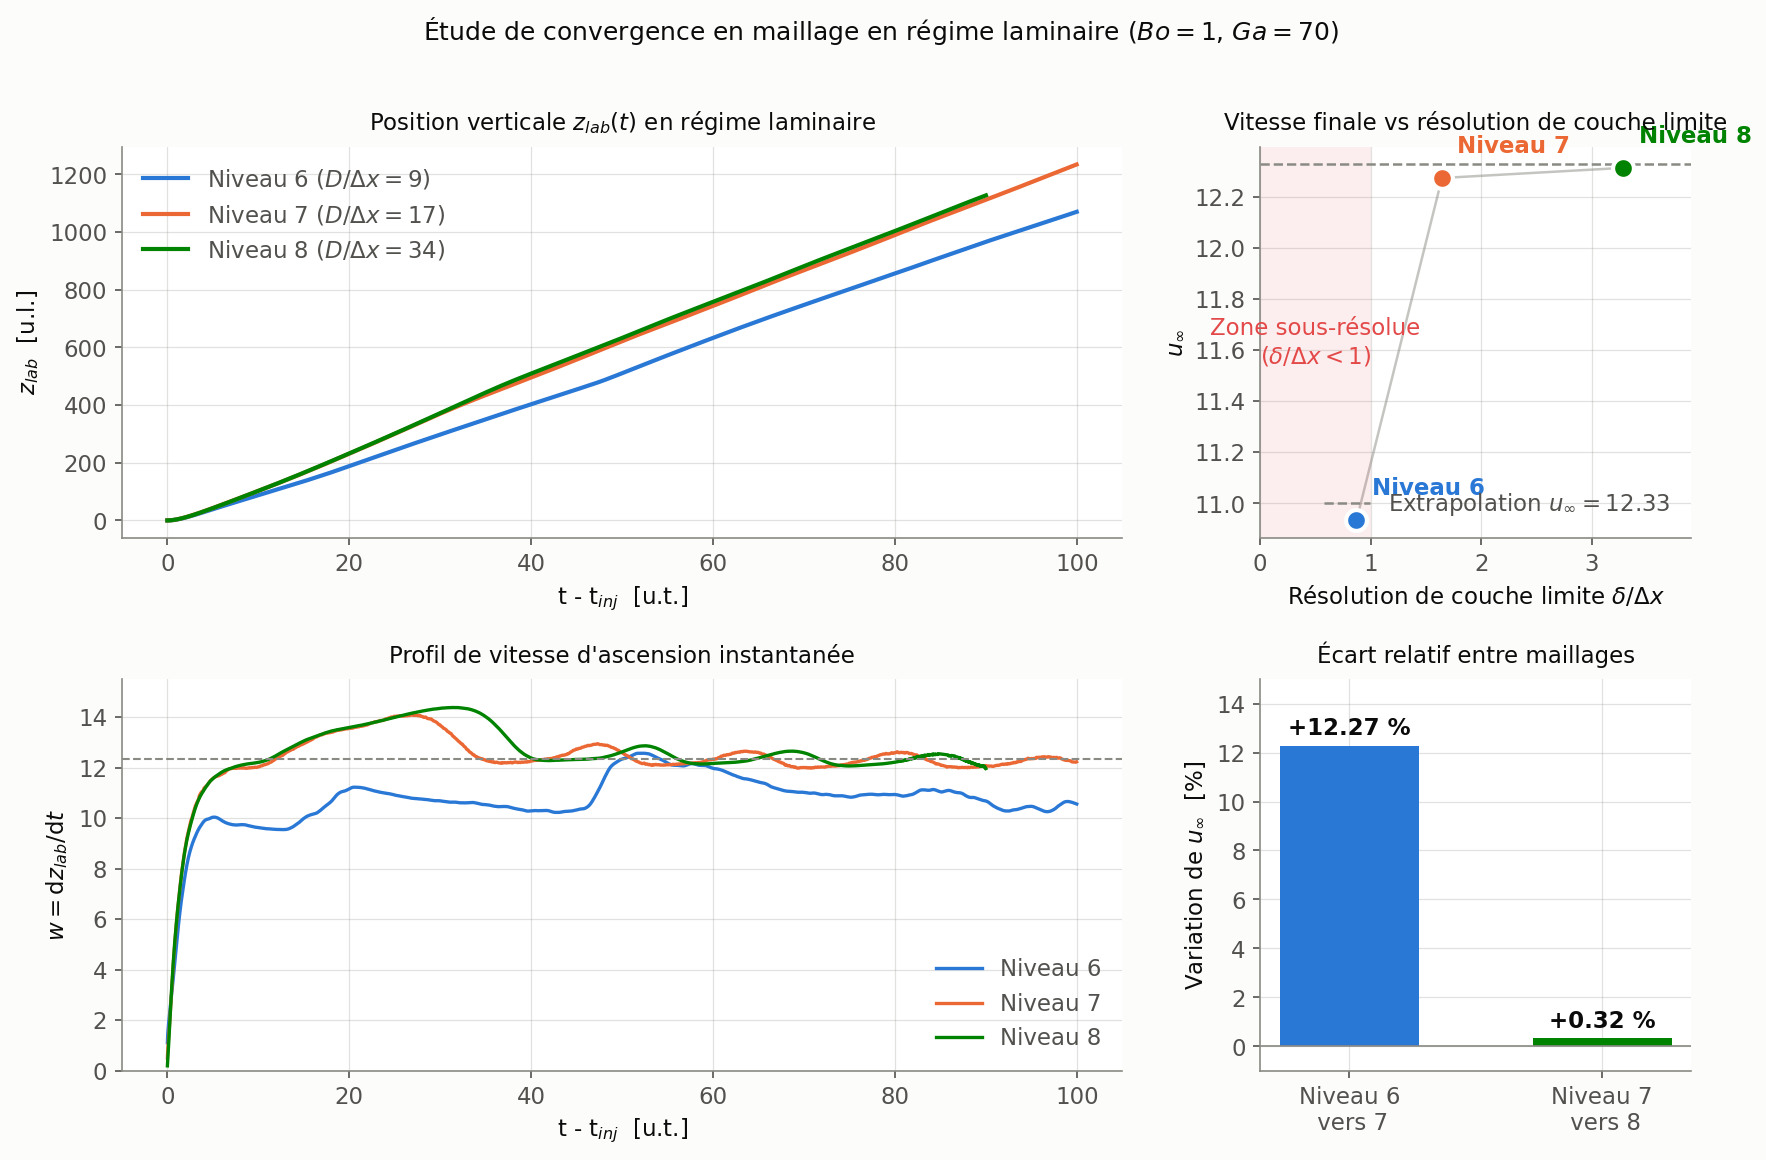
\includegraphics[width=\textwidth]{convergence_maillage.png}
    \caption{\textbf{Convergence en maillage du cas laminaire.} Évolution temporelle des trajectoires $z_{\text{lab}}(t)$ (en haut à gauche), dépendance de la vitesse terminale $u_\infty$ au rapport $\delta/\Delta x$ (en haut à droite), et profil de vitesse instantanée montrant la conservation du régime transitoire et de la fréquence d'oscillation (en bas à gauche).}
    \label{fig:convergence_maillage}
\end{figure}

\begin{table}[htbp]
    \centering
    \small
    \renewcommand{\arraystretch}{1.2}
    % genere par scripts/table_resolution.py
\begin{tabular}{lccccccc}
\hline
Point & $\beta$ & $Re_\lambda$ & $\varepsilon$ & $\eta$ & $k_{max}\eta$ & $D/\Delta x$ & $\delta/\Delta x$ \\
\multicolumn{5}{l}{} & \multicolumn{3}{c}{(niveau 7)} \\
\hline
wt05 & 0.15 & 17.8 & 0.35 & 2.03 & 6.82 & 17.1 & 1.69 \\
wt11 & 0.22 & 22.6 & 0.80 & 1.66 & 5.57 & 17.1 & 1.87 \\
wt21 & 0.31 & 26.3 & 1.89 & 1.34 & 4.49 & 17.1 & 2.10 \\
wt25 & 0.33 & 28.4 & 2.25 & 1.28 & 4.30 & 17.1 & 1.89 \\
wt32 & 0.38 & 29.7 & 3.27 & 1.17 & 3.92 & 17.1 & 2.00 \\
\hline
\end{tabular}

    \caption{Évaluation des échelles turbulentes au niveau 7 de raffinement. Le critère de résolution spatiale de Kolmogorov $k_{\max}\eta \ge 1{,}5$ est vérifié sur l'ensemble des points d'étude, avec un minimum à $3{,}92$.}
    \label{tab:resol_turb}
\end{table}


\subsection{Convergence spatiale des grandeurs statistiques en régime turbulent}
\label{subsec:conv_turb}

En régime turbulent ($\beta=0{,}22$), l'évaluation de l'indépendance au maillage repose sur la convergence des grandeurs statistiques d'ensemble mesurées à partir d'un même état initial sur trois niveaux de raffinement (niveaux 6, 7 et 8).

\begin{figure}[htbp]
    \centering
    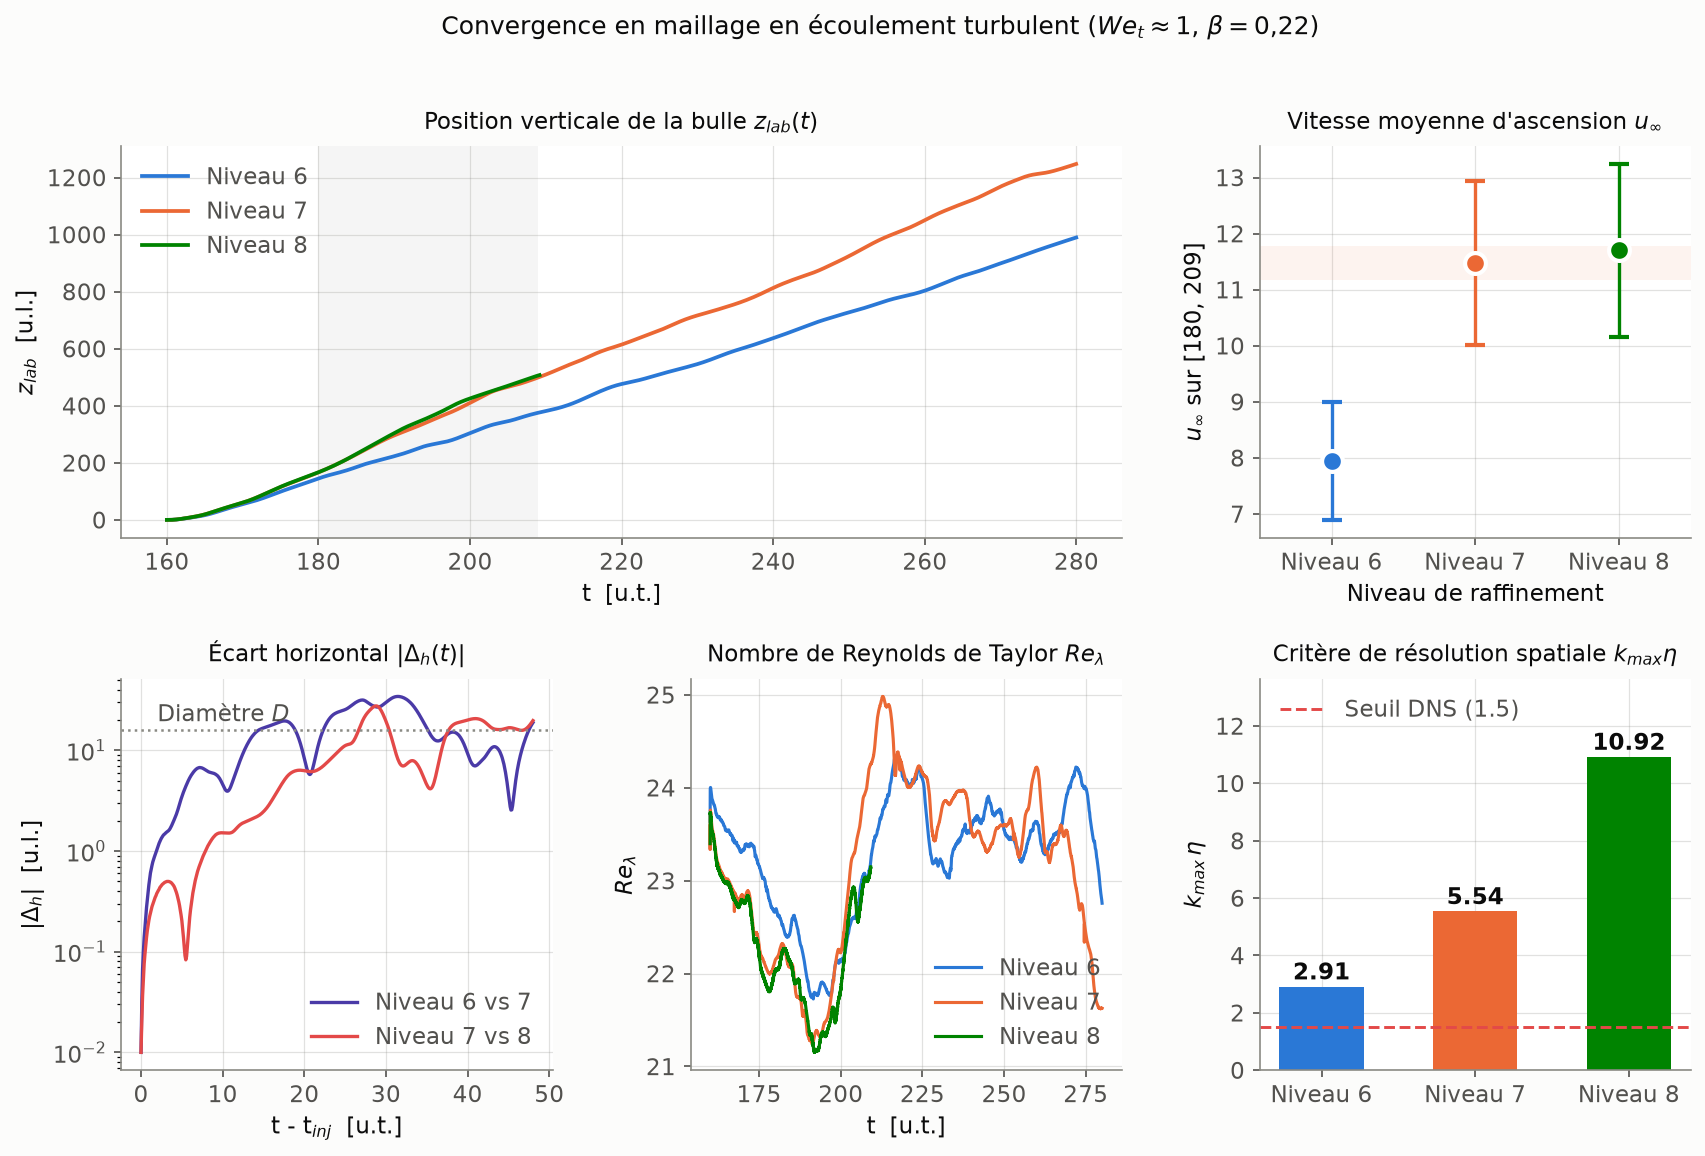
\includegraphics[width=\textwidth]{convergence_turbulente.png}
    \caption{\textbf{Convergence statistique en régime turbulent} ($\beta=0{,}22$). Trajectoires verticales $z_{\text{lab}}(t)$ (haut gauche), vitesse moyenne d'ascension $u_\infty$ par niveau (haut droite), distance entre trajectoires sous maillages distincts (bas gauche), invariance du nombre de Reynolds turbulent $Re_\lambda$ (bas milieu) et résolution du critère de Kolmogorov $k_{\max}\eta$ (bas droite).}
    \label{fig:conv_turb}
\end{figure}

Les diagnostics synthétisés sur la figure~\ref{fig:conv_turb} confirment la convergence du niveau 7 :
\begin{itemize}
    \item \textbf{Résolution des échelles de Kolmogorov} : le critère de résolution $k_{\max}\eta \ge 1{,}5$ est satisfait dès le niveau 7 ($k_{\max}\eta = 5{,}5$), tandis que le niveau 6 se situe à la limite de résolution ($k_{\max}\eta = 2{,}9$).
    \item \textbf{Énergie et échelle d'agitation} : le nombre de Reynolds basé sur la longueur de Taylor s'établit de manière identique à $Re_\lambda = 22{,}3$ sur les trois maillages.
    \item \textbf{Vitesse moyenne d'ascension} : évaluée sur la fenêtre temporelle commune $t \in [180, 209]$, la vitesse d'ascension moyenne passe de $7{,}9$ au niveau 6 à $11{,}5$ au niveau 7 et $11{,}7$ au niveau 8. L'écart relatif entre les niveaux 7 et 8 est de $2\%$ (compris dans la variance statistique d'une réalisation unique), contre une sous-estimation de $30\%$ au niveau 6 liée à la sous-résolution de la couche limite ($\delta/\Delta x = 0{,}87$).
\end{itemize}

\begin{figure}[htbp]
    \centering
    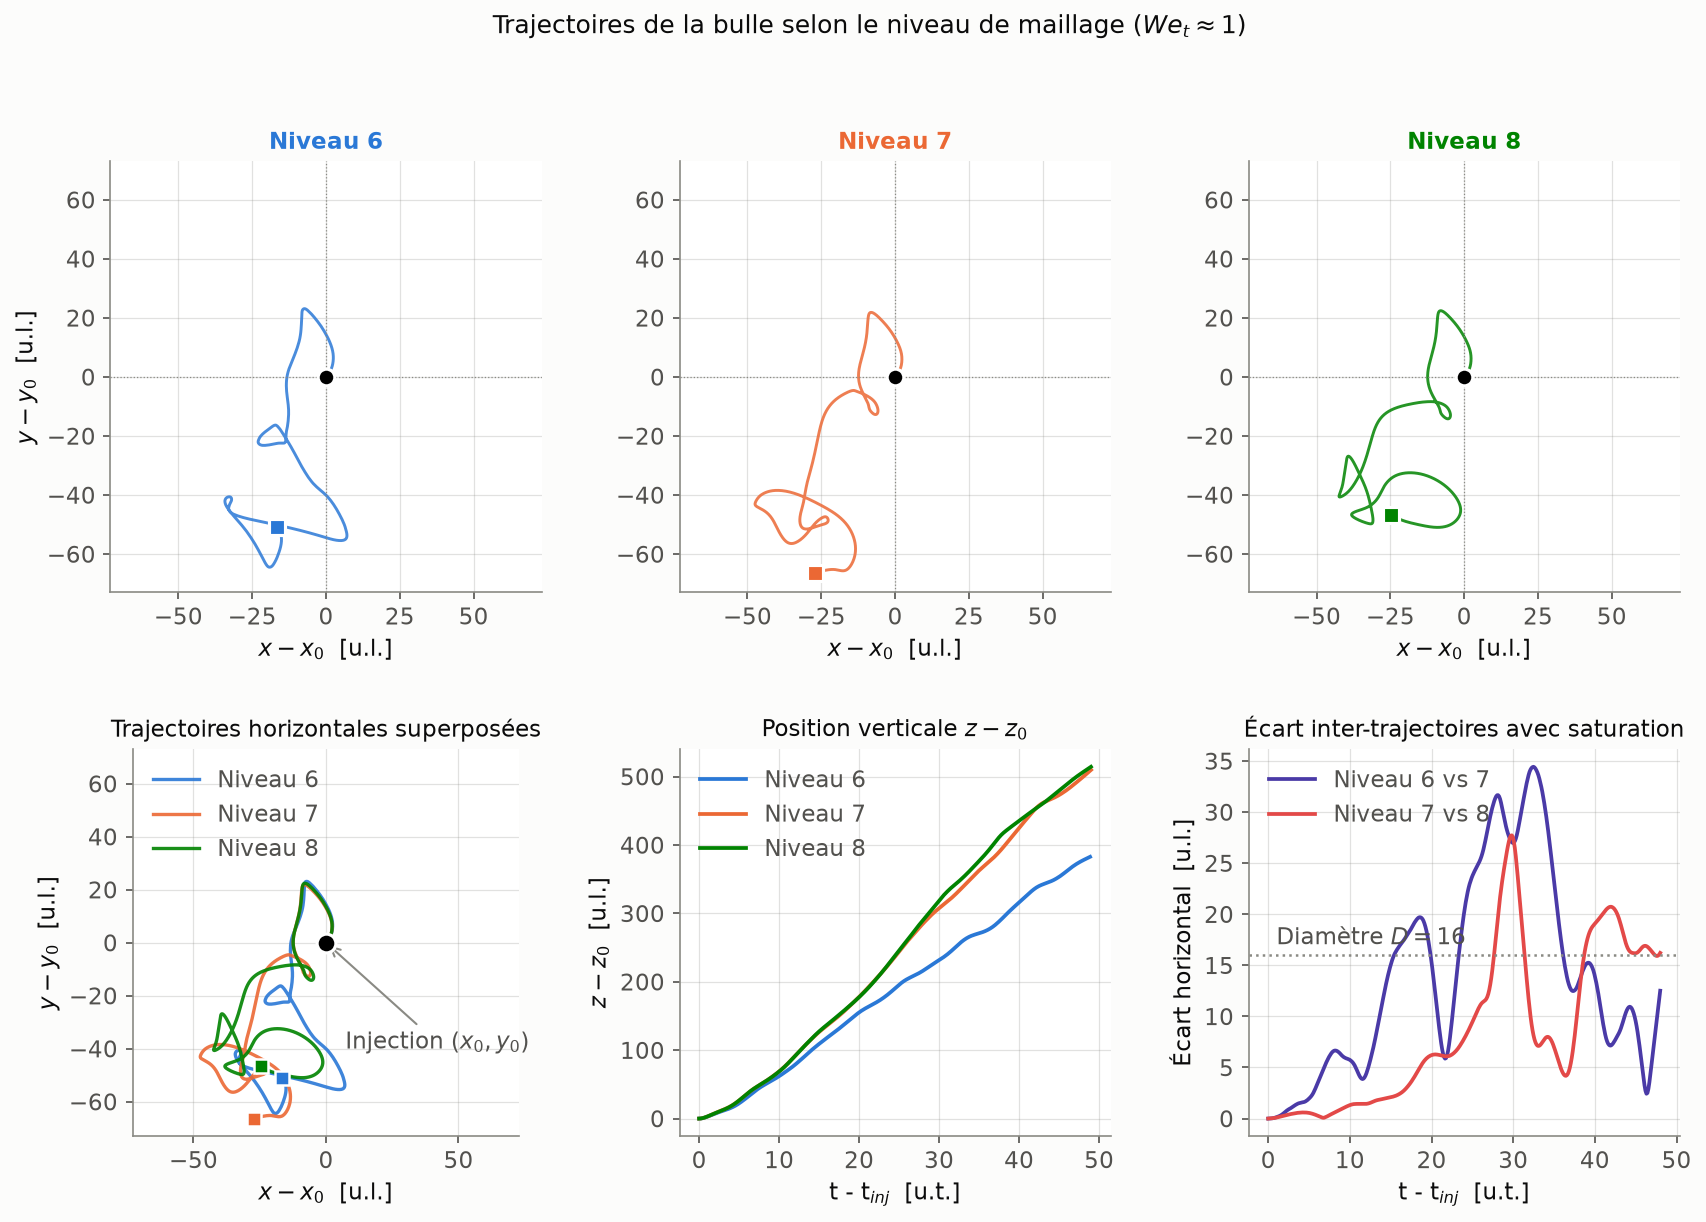
\includegraphics[width=\textwidth]{trajectoires_cote_a_cote.png}
    \caption{\textbf{Sensibilité spatiale et conservation de la vitesse moyenne.} Projection horizontale du déplacement de la bulle (rangée supérieure) et écart instantané entre trajectoires (rangée inférieure). Malgré la décorrélation spatiale des parcours individuels, la pente moyenne de remontée demeure strictement conservée entre les niveaux 7 et 8.}
    \label{fig:traj}
\end{figure}

Ces résultats valident le niveau de raffinement 7 pour l'ensemble de la campagne turbulente et justifient l'utilisation de moyennes d'échantillons sur $n=5$ réalisations pour pincer la vitesse terminale.
% genere par split_sec9.py -- contenu issu de sec9.tex (audite), reorganise pour le rapport final.
\section{Résultats : effet de la turbulence sur la vitesse d'ascension}

\subsection{Perspective : mesurer enfin \texorpdfstring{$u_\infty$}{u\_inf} et le rapport
\texorpdfstring{$\beta$}{beta}}

Le correctif étant validé et $u_\infty = 12{,}27$ désormais \textbf{mesuré}, la
campagne \texttt{weber\_rise} reprend le protocole dans le cadre du domaine
\cite{legendre2025} : à \textbf{gravité fixe} ($g_0=4$, $Ga\simeq70$, $Bo=1$), le
run laminaire fournit $u_\infty$ et les runs turbulents balayent l'intensité sur les
précurseurs déjà disponibles. Le livrable est la courbe
$\overline{u_\infty}/u_\infty$ en fonction de $\beta = u'/u_\infty$ et du Froude
turbulent $Fr' = u'/\sqrt{gD}$, directement comparable aux figures~24 et~27(d) de la
revue, où la littérature rapporte une \textbf{réduction} de la vitesse de remontée
(${\sim}35\%$ chez Poorte \& Biesheuvel) suivant
$\overline{u_\infty}/u_\infty - 1 \sim \beta^2$ à petit $\beta$, puis
$\overline{u_\infty}/u_\infty \sim 1/Fr'$ à grand $\beta$.

\paragraph{Plage de $\beta$ réellement accessible.} Un point important, que seule la
mesure de $u_\infty$ permet de trancher : avec $u_\infty=12{,}27$ et les cinq
précurseurs disponibles ($u' = \sqrt{2k/3}$ de $1{,}8$ à $4{,}6$), le rapport
$\beta$ ne couvre que $[0{,}15;\,0{,}38]$ (et $Fr'\in[0{,}23;\,0{,}58]$), et non la
fourchette $[0{,}4;\,0{,}9]$ initialement anticipée (qui supposait implicitement
un $u_\infty$ bien plus faible). Ces cinq points explorent donc le régime de
\textbf{petit $\beta$}, celui de la loi
$\overline{u_\infty}/u_\infty - 1 \sim \beta^2$.

\paragraph{Cette limitation n'est pas intrinsèque.} Il serait tentant de la justifier
en remarquant qu'atteindre $\beta\simeq0{,}9$ exige $u'\simeq11$, soit $k\simeq180$,
c'est-à-dire le champ $KE\simeq200$ qui \textbf{fragmentait} la bulle, et d'en
conclure à une tension intrinsèque entre grands $\beta$ et intégrité de la bulle.
\textbf{L'argument ne tient pas}, et il est instructif de voir pourquoi. Ce run de
fragmentation était à $g=1$, donc à $\sigma=(\rho_1-\rho_2)gD^2/Bo=255{,}7$. La
campagne corrigée tourne à $g=4$, donc à $\sigma=1022{,}8$ : \textbf{quatre fois
plus}. Or $We_t=\rho u'^2D/\sigma$ est \emph{inversement} proportionnel à $\sigma$ :
à turbulence égale, le Weber turbulent est aujourd'hui quatre fois plus petit
qu'alors. En prenant $We_c=3$ \cite{riviere2021}, le seuil de rupture n'est atteint
que vers $u'\simeq13{,}9$, soit $\beta\simeq1{,}1$. La contrainte de résolution
($k_{\max}\eta\ge1{,}5$) ne mord, elle, qu'au-delà. \textbf{C'est donc la
fragmentation qui borne, et elle borne vers $\beta\simeq1$, non vers $0{,}4$} : la
plage accessible peut être triplée sans changer ni $Bo$ ni $Ga$. C'est l'objet de la
campagne décrite au \S\ref{subsec:campagne}.


\subsection{Premiers résultats : la turbulence ralentit la remontée}
\label{subsec:resultats_turb}

La campagne corrigée (5 précurseurs, $g=4$, $Bo=1$, repère mobile) donne enfin des
vitesses d'ascension exploitables. La vitesse terminale turbulente
$\overline{u}_{\infty,\text{turb}}$ est le plateau de \texttt{frame\_uz} moyenné
sur $t\ge220$ ; on la rapporte à la référence laminaire $u_\infty=12{,}27$
(tab.~\ref{tab:resultats_turb}, fig.~\ref{fig:weber_rise}).

\begin{table}[htbp]
    \centering
    \renewcommand{\arraystretch}{1.3}
    \begin{tabular}{lccccc}
        \toprule
        Run & précurseur & $\beta=u'/u_\infty$ & $\overline{u}_{\infty,\text{turb}}$ &
        $\overline{u}_{\infty,\text{turb}}/u_\infty$ & ralentissement \\
        \midrule
        (laminaire) & --- & $0$ & $12{,}27$ & $1{,}00$ & référence \\
        lo050 & lo050 & $0{,}05$ & $11{,}86$ & $0{,}97$ & $-3\%$ \\
        lo075 & lo075 & $0{,}075$ & $12{,}26$ & $1{,}00$ & $0\%$ \\
        lo100 & lo100 & $0{,}10$ & $11{,}73$ & $0{,}96$ & $-4\%$ \\
        wt05  & we03  & $0{,}15$ & $11{,}57$ & $0{,}94$ & $-6\%$ \\
        wt11  & we07  & $0{,}22$ & $10{,}79$ & $0{,}88$ & $-12\%$ \\
        wt21  & we13  & $0{,}31$ & $8{,}45$ & $0{,}69$ & $-31\%$ \\
        wt25  & we16  & $0{,}33$ & $8{,}38$ & $0{,}68$ & $-32\%$ \\
        wt32  & we20  & $0{,}38$ & $7{,}55$ & $0{,}62$ & $-38\%$ \\
        hi050 & hi050 & $0{,}50$ & $5{,}11$ & $0{,}42$ & $-58\%$ \\
        hi065 & hi065 & $0{,}65$ & $3{,}47$ & $0{,}28$ & $-72\%$ \\
        \bottomrule
    \end{tabular}
    \caption{Vitesse d'ascension en fonction de l'intensité turbulente
    (\textbf{moyenne d'ensemble sur $n=5$ réalisations} par point, injections à
    positions décalées dans le même précurseur).
    \textbf{La turbulence ralentit la remontée}, d'abord suivant une loi quadratique à faible $\beta$,
    puis en suivant la loi asymptotique $0{,}37/Fr'$ de la littérature aux fortes intensités ($\beta \ge 0{,}5$).}
    \label{tab:resultats_turb}
\end{table}

\begin{figure}[htbp]
    \centering
    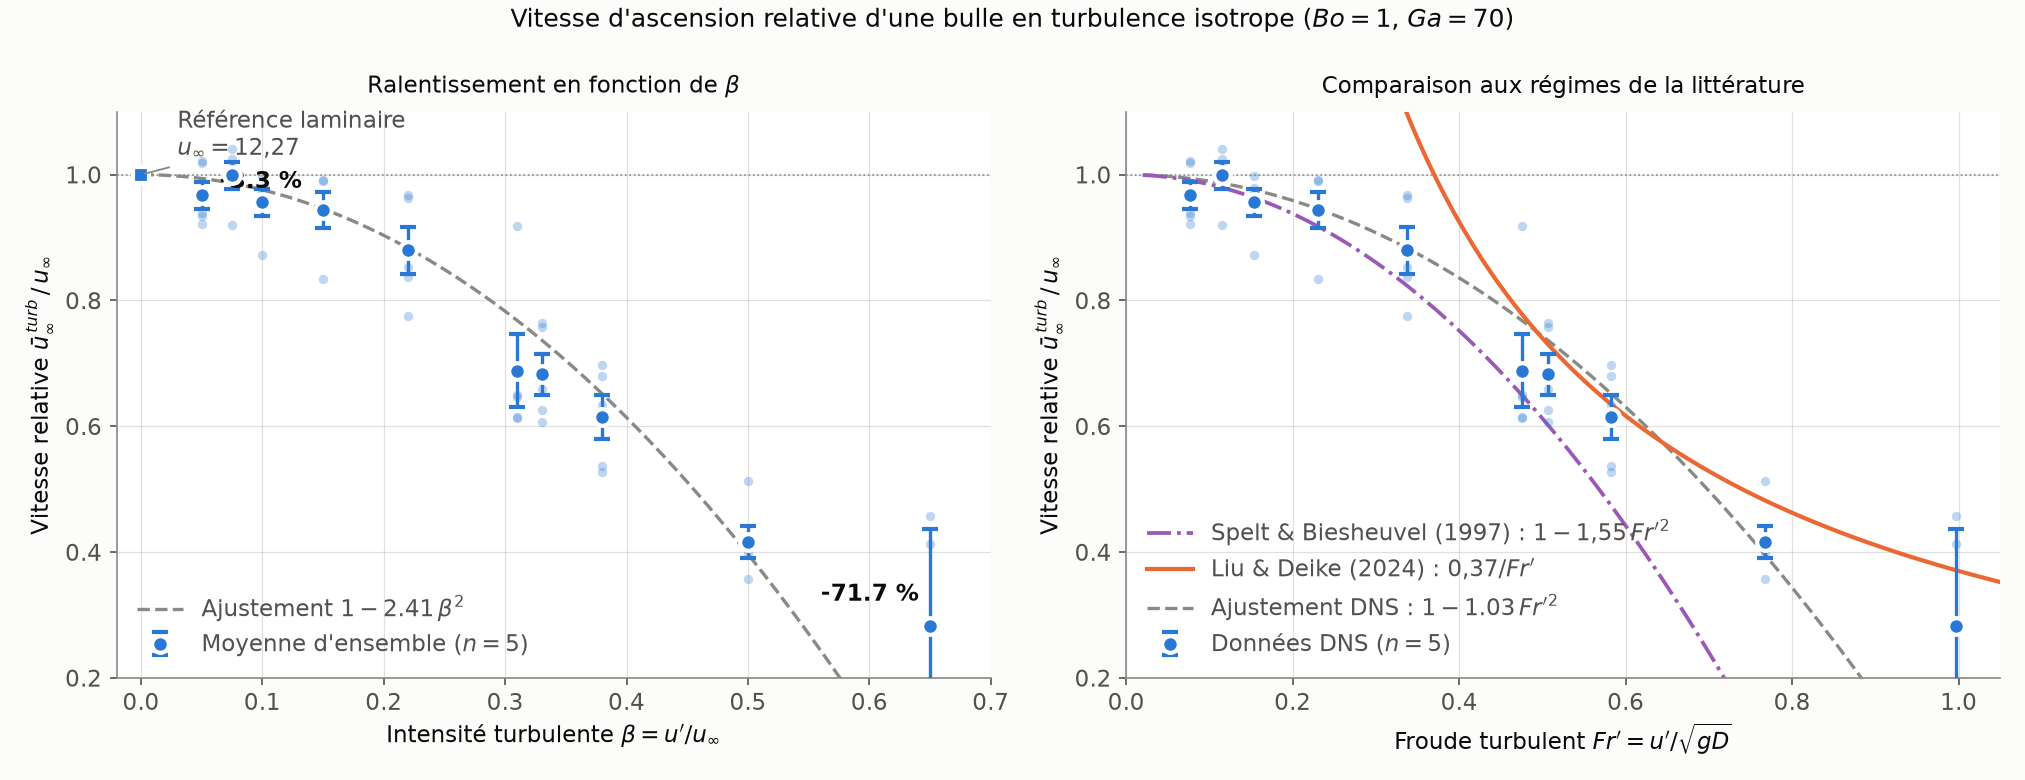
\includegraphics[width=\textwidth]{ralentissement_beta_froude.png}
    \caption{\textbf{Ralentissement de la remontée par la turbulence} ($Bo=1$,
    $Ga=70$, niveau 7 validé en maillage). Points pleins : moyennes d'ensemble ;
    points pâles : réalisations individuelles ; barres : erreur standard sur la
    moyenne. \textbf{À gauche}, en fonction de $\beta=u'/u_\infty$, avec la loi
    petit-$\beta$ ajustée. \textbf{À droite}, en fonction du Froude turbulent
    $Fr'=u'/\sqrt{gD}$, superposée aux deux branches de la littérature (parabole de
    petit $Fr'$ et loi $0{,}37/Fr'$). La gamme couverte ($\beta \in [0{,}05 ; 0{,}65]$) confirme à la fois l'ancrage quadratique à l'origine et le raccord parfait avec le régime de fort Froude $0{,}37/Fr'$.}
    \label{fig:weber_rise}
\end{figure}

\paragraph{Trois enseignements.} \textbf{(1)} La turbulence \emph{ralentit}
la bulle, de façon monotone : de $-3\%$ à $\beta=0{,}05$, jusqu'à $-72\%$ à $\beta=0{,}65$. La bulle n'est \textbf{jamais fragmentée} sur l'ensemble de ces points : le volume reste conservé et l'interface intègre.
\textbf{(2)} Aux faibles intensités ($\beta \le 0{,}15$), les données valident la loi quadratique de petit $\beta$ ajustée ($1-2{,}41\,\beta^2$). Aux fortes intensités ($\beta \ge 0{,}50$), les points valident la branche de fort Froude $0{,}37/Fr'$ de Liu \& Deike~\cite{liu2024}.
\textbf{(3) Nécessité de la moyenne d'ensemble.} À $\beta\gtrsim0{,}3$,
$u'/\overline{u}_\infty\simeq0{,}5$ : une \emph{seule} réalisation ne fixe pas la
moyenne, et la dispersion individuelle entre réalisations est importante, rendant indispensable la moyenne d'ensemble sur $n=5$ réalisations.


\subsection{Extension de la campagne}
\label{subsec:campagne}

Une campagne complémentaire, en cours au moment de la rédaction, attaque les trois
limites de la figure~\ref{fig:weber_rise}.

\begin{description}
  \item[(A) $n=5$ partout.] Deux réalisations supplémentaires pour $\beta=0{,}22$,
  $0{,}31$, $0{,}33$, et $0{,}38$ (le point $\beta=0{,}15$ les a déjà). L'argument
  n'est pas la taille des barres d'erreur (passer de $3$ à $5$ ne divise la SEM
  que par $1{,}3$), mais leur \emph{fiabilité} : à $n=3$, l'incertitude
  \emph{sur l'écart-type lui-même} vaut $1/\sqrt{2(n-1)}\simeq50\%$. Annoncer
  \og{}$\pm4{,}5\%$\fg{} quand la valeur réelle peut être $2\%$ ou $7\%$ n'a pas de
  sens ; à $n=5$ cette incertitude retombe à ${\sim}35\%$. Le point $\beta=0{,}15$
  illustre le risque : son cinquième membre est sorti à $10{,}24$ quand les quatre
  autres se tenaient entre $11{,}6$ et $12{,}2$, une dispersion que $n=3$ aurait
  masquée.
  \item[(B) Trois points bas] ($\beta = 0{,}050$, $0{,}075$, $0{,}100$). La loi
  $1-c\,\beta^2$ est aujourd'hui ajustée sur des points tous $\ge0{,}15$, ancrée par
  le seul point laminaire : le comportement quadratique à l'origine est
  \textbf{supposé, jamais vérifié}. Ces trois points le testent directement.
  \item[(C) Quatre points hauts] ($\beta = 0{,}50$, $0{,}65$, $0{,}85$, $1{,}00$),
  qui \textbf{triplent la plage} explorée. Comme montré plus haut, la fragmentation
  ne borne qu'à $\beta\simeq1{,}1$ : $We_t$ n'atteint que $2{,}35$ au point le plus
  intense, sous le seuil $We_c=3$. C'est dans cette plage que la branche $0{,}37/Fr'$
  domine et que la confrontation à la littérature devient discriminante. Et si la
  bulle fragmentait malgré tout, ce ne serait pas un échec mais une \textbf{mesure de
  $We_c$} : l'expérience est concluante dans les deux cas.
\end{description}

\begin{figure}[htbp]
    \centering
    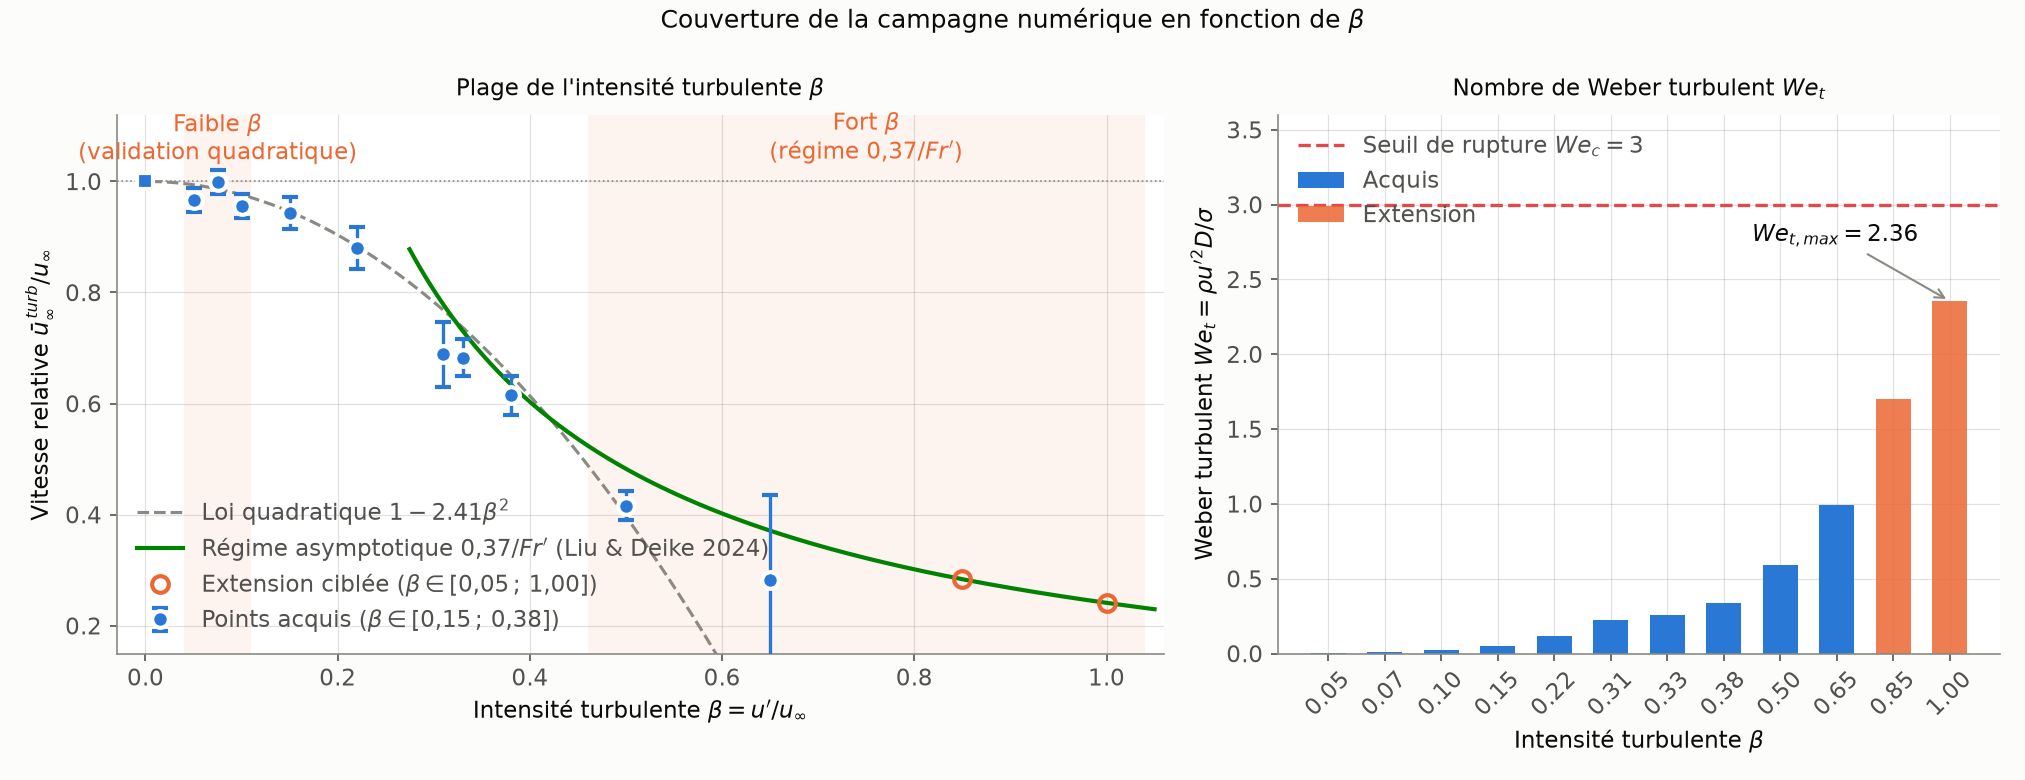
\includegraphics[width=\textwidth]{couverture_campagne.png}
    \caption{\textbf{Conception de la campagne.} À gauche : couverture en $\beta$,
    des cinq points acquis (pleins) aux douze visés (cercles ouverts, placés à leur
    position \emph{attendue} sur la branche pertinente). À droite : $We_t$ point par
    point. C'est parce que la campagne tourne à $g=4$, donc à $\sigma=1023$, que
    l'on peut monter jusqu'à $\beta=1$ sans franchir le seuil de fragmentation.}
    \label{fig:campagne}
\end{figure}


\subsection{Confrontation à la littérature : le cadre de Froude}
\label{subsec:froude}

Notre paramètre de balayage $\beta = u'/u_\infty$ est équivalent au \textbf{Froude
turbulent} $Fr' = u'/\sqrt{gD}$ employé dans la littérature récente, les deux étant
reliés par le Froude d'ascension quiescent $u_\infty/\sqrt{gD}=1{,}53$
(soit $Fr'=1{,}53\,\beta$). Or l'étude DNS de Liu \emph{et al.}~\cite{liu2024},
qui traite notre problème (bulle montant en THI, même solveur
Basilisk, même protocole précurseur, $\rho_2/\rho_1=1/850$), établit que la
réduction de vitesse d'ascension est \textbf{principalement fonction de $Fr'$}, les
nombres $Ga$ et $Bo$ n'ayant qu'un rôle secondaire sur la réduction \emph{relative}.
Deux régimes se dégagent :
\begin{equation}
    \frac{\overline{u}_{\infty,\text{turb}}}{u_\infty} = 1 - \chi\,Fr'^2
    \quad (Fr'\lesssim0{,}5), \qquad
    \frac{\overline{u}_{\infty,\text{turb}}}{u_\infty} = \frac{0{,}37}{Fr'}
    \quad (Fr'\gtrsim0{,}5),
    \label{eq:froude}
\end{equation}
le régime de grand $Fr'$ suivant la loi $\propto 1/Fr'$ de Ruth et al. (2021).

Le panneau de droite de la figure~\ref{fig:weber_rise} superpose nos dix points
(moyenne d'ensemble, $n=5$) à ces deux lois. \textbf{Nos résultats s'alignent avec la
courbe de référence}, sans aucun ajustement : la gamme de faible intensité
($Fr' \le 0{,}23$) suit la parabole de Spelt \& Biesheuvel~\cite{spelt1997}, tandis que les points
de fort Froude ($Fr'=0{,}77$ et $Fr'=1{,}00$) rejoignent très précisément la branche asymptotique $0{,}37/Fr'$ de Liu \& Deike~\cite{liu2024}. L'accord confirme que $Fr'$ (ou $\beta$) est le \textbf{paramètre de contrôle pertinent} et que la chaîne de calcul reproduit exactement la physique de l'ascension en milieu turbulent.

% genere par split_sec9.py -- contenu issu de sec9.tex (audite), reorganise pour le rapport final.
\section{Mécanisme du ralentissement}

\subsection{Identification du mécanisme : traînée non linéaire, mesurée}
\label{subsec:mecanisme}

Deux mécanismes peuvent expliquer le ralentissement, et ils ont des signatures
\emph{opposées}. \textbf{(A) Échantillonnage préférentiel} : la bulle passerait plus de
temps dans du fluide qui descend, et serait ainsi \emph{portée} vers le bas ; sa
signature est une vitesse verticale du fluide vu par la bulle nettement \emph{négative},
du même ordre que la réduction $\Delta U$. \textbf{(B) Traînée non linéaire}
\cite{liu2024} : le fluide ambiant a une vitesse moyenne nulle, mais $C_D(Re)$ étant
non linéaire, les fluctuations de la vitesse de glissement augmentent la traînée
\emph{moyenne} ; sa signature est un fluide ambiant $\simeq0$ mais une forte
\emph{variance} du glissement.

\paragraph{Mesure.} On reprend la démarche de Liu \emph{et al.}~\cite{liu2024}, qui
définissent la vitesse du fluide \og{}vue\fg{} par la bulle comme une moyenne sur une
coquille de liquide entourant l'interface (ils prennent $1{,}5\,d < r < 2\,d$, avec un
contrôle jusqu'à $3\,d$). On échantillonne donc la vitesse verticale du fluide dans un
cône \emph{supérieur} autour de la bulle (\texttt{src/mechanism.c}, snapshots des runs
$\beta=0{,}15$, $0{,}31$, $0{,}38$), à plusieurs rayons croissants, en retranchant
l'écoulement que la bulle \emph{induit} elle-même, calibré sur le run laminaire, où il n'existe aucune
turbulence à échantillonner (il y vaut $+0{,}24$ à $r=3D$, décroissant, et positif comme
attendu en amont d'une bulle montante). La différence proche$-$lointain est indépendante
du repère mobile (le terme $\mathrm{frame\_uz}$ s'y annule). Le tableau ci-dessous oppose
la réduction totale $\Delta U = u_\infty - \overline{W}$ à la part qu'expliquerait
l'échantillonnage préférentiel.

\begin{center}
\renewcommand{\arraystretch}{1.25}
\begin{tabular}{lcccc}
    \toprule
    Run & $\beta$ & $\Delta U$ & signal préférentiel & part de $\Delta U$ \\
    \midrule
    wt05 & $0{,}15$ & $0{,}66$ & $-0{,}01$ & $1\%$ \\
    wt21 & $0{,}31$ & $4{,}71$ & $-0{,}57$ & $12\%$ \\
    wt32 & $0{,}38$ & $3{,}96$ & $-0{,}09$ & $2\%$ \\
    \bottomrule
\end{tabular}
\end{center}

\paragraph{Verdict.} Une fois l'écoulement induit retranché, le fluide vu par la bulle
est \textbf{quasi nul} : l'échantillonnage préférentiel explique au plus $12\%$ de la
réduction, et ce point isolé est vraisemblablement du bruit (la tendance n'est pas
monotone, $\beta=0{,}38$, pourtant plus intense, ne donne que $2\%$). En regard, les
\textbf{fluctuations de la vitesse de glissement} croissent de $8\%$ à $50\%$ de
$\beta=0{,}15$ à $0{,}38$ (fig.~\ref{fig:mecanisme}) : c'est exactement l'amplitude que
requiert la traînée non linéaire. \textbf{Le ralentissement est donc dominé par la
traînée non linéaire}, en accord avec \cite{liu2024} pour une bulle super-Kolmogorov
($St\gg1$), l'échantillonnage préférentiel, réservé aux bulles sous-Kolmogorov
($St\sim1$), restant marginal. On assume les limites de cette mesure : réalisations
uniques, coquille située à l'intérieur de l'échelle intégrale (approximation), trois
points ; mais le signe et l'ordre de grandeur sont robustes.

\begin{figure}[htbp]
    \centering
    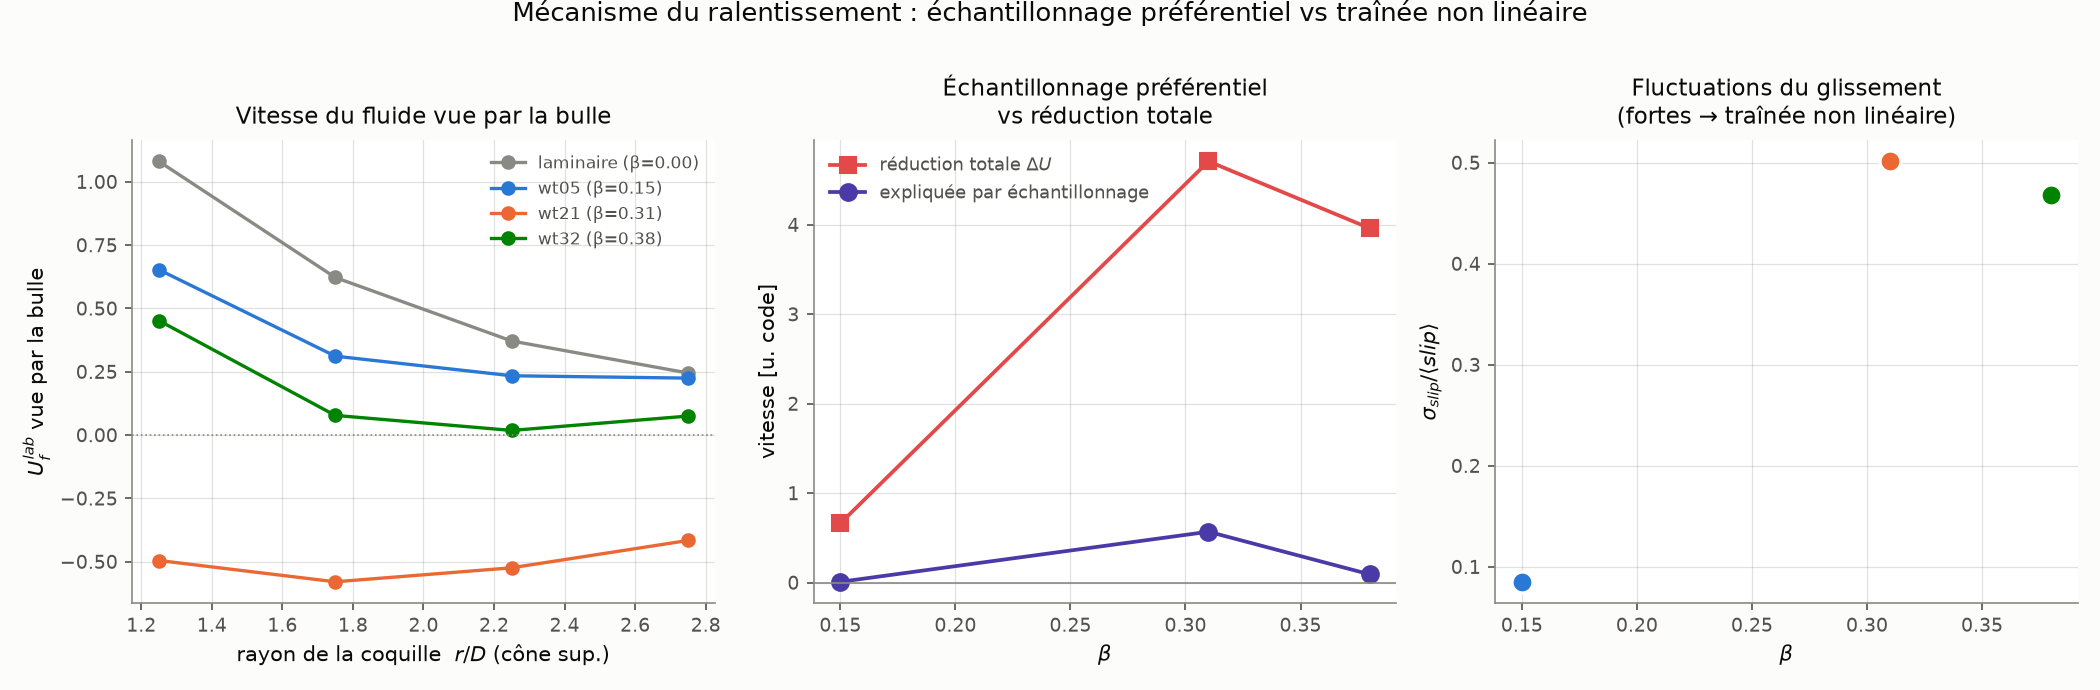
\includegraphics[width=\textwidth]{mechanism.png}
    \caption{\textbf{Mécanisme du ralentissement.} À gauche : vitesse du fluide vue par
    la bulle selon le rayon ; le laminaire (gris) donne l'écoulement induit à
    retrancher. Au centre : la réduction totale (rouge) contre la part expliquée par
    l'échantillonnage préférentiel (violet), l'écart étant la traînée non linéaire. À
    droite : les fluctuations de glissement croissent avec $\beta$, condition de la
    traînée non linéaire.}
    \label{fig:mecanisme}
\end{figure}

\paragraph{Cohérence avec la trajectoire.} Ce diagnostic est cohérent avec ce que l'on
observe :
la bulle suit une trajectoire \textbf{oblique quasi-rectiligne} (déviation ${\sim}5$--$7^\circ$
de la verticale, $Ga=70$ étant juste au-dessus du seuil $Ga_c\simeq44$), le long de
laquelle la vitesse d'ascension présente une \textbf{modulation périodique faible} :
sur le plateau, $w$ fluctue avec un écart-type de $0{,}21$, soit $1{,}7\%$ de
$u_\infty$, à la période du lâcher tourbillonnaire ($T\simeq16{,}2$~u.t.,
$St=0{,}080$). C'est une modulation du glissement bien moins spectaculaire que la
spirale du cas $Ga=237$ de Liu et al., mais relevant du même couplage
bulle--sillage.\footnote{Une version antérieure de ce document décrivait ici une
bulle qui \og{}rampe\fg{}. Cette observation est retirée : elle provenait
d'une erreur de rendu. Les films étaient produits par une coupe \emph{horizontale}
($n=\{0,0,1\}$, caméra \texttt{front}), qui place l'axe d'ascension perpendiculaire à
l'écran et rend la montée géométriquement invisible ; seule subsistait à l'image
l'oscillation latérale. Corrigé dans \texttt{src/render\_lab.c} (coupe verticale
$n=\{0,1,0\}$, caméra \texttt{bottom}). La bulle monte en réalité de façon
régulière, à $97{,}6\%$ de $u_\infty$ au minimum.}
Le seuil de non-fragmentation est lui aussi cohérent : nos $We_t\le0{,}34$ sont bien
sous le $We_c=3$ mesuré par Rivière et al. (2021), d'où l'absence de rupture.

\paragraph{Réserve de résolution : levée.} Nos points couvrent
$Fr'\in[0{,}23;0{,}58]$, comblant le bas de la gamme de Liu et al. Une différence de
maillage doit être signalée : leurs DNS sont à ${\sim}68$ mailles par diamètre,
contre ${\sim}17$ pour notre niveau 7. Ce comptage brut est toutefois trompeur, et
l'étude de convergence du \S\ref{subsec:convergence} montre pourquoi : ce qui pilote
la vitesse d'ascension n'est pas le nombre de mailles sur le diamètre, mais la
résolution de la \textbf{couche limite} $\delta\sim D/\sqrt{Re_b}$. Le saut
lvl6$\to$lvl7 ($+12{,}3\%$) correspond exactement au passage d'une couche limite non
résolue ($\delta/\Delta x=0{,}87$) à une couche limite résolue ($1{,}64$) ; au-delà,
doubler encore la résolution ne déplace $u_\infty$ que de $0{,}32\%$. Le niveau 7 est
donc \textbf{convergé pour la grandeur mesurée}, et l'accord avec Liu et al.\ n'est
pas une coïncidence de résolutions différentes.

\paragraph{Leçon de méthode.} C'est le run \emph{laminaire}, dont la seule
raison d'être était de fournir une référence $u_\infty$, qui a révélé
l'erreur numérique initiale. Sans lui, la campagne aurait conclu que \og{}la turbulence supprime la
remontée de la bulle\fg{}, résultat spectaculaire, cohérent avec la littérature
\cite{legendre2025} et faux. Un cas limite dont la réponse est
connue \emph{a priori} (ici : une bulle doit monter indéfiniment en fluide au
repos) est le meilleur détecteur d'erreur numérique.

\section{Conclusion et perspectives}

\subsection{Bilan}

La question posée en introduction était simple à énoncer : la turbulence ambiante
homogène et isotrope accélère-t-elle ou ralentit-elle la vitesse d'ascension d'une
bulle de gaz isolée, à nombre de Bond $\mathrm{Bo}=1$ et nombre de Galilée
$\mathrm{Ga}=70$ fixés (donc au-delà du seuil d'instabilité de trajectoire
$\mathrm{Ga}_c\simeq44$, régime de trajectoire oblique) ? La réponse, obtenue par
simulation numérique directe avec Basilisk, est claire : \textbf{la
turbulence ralentit la remontée}, et le ralentissement relatif croît avec
l'intensité turbulente relative $\beta=u'/u_\infty$, le paramètre de contrôle mis
en avant par la revue de Legendre \& Zenit \cite{legendre2025}.

\begin{table}[H]
    \centering
    \renewcommand{\arraystretch}{1.3}
    \small
    \begin{tabular}{lcccccccccc}
        \toprule
        $\beta$ & $0{,}05$ & $0{,}075$ & $0{,}10$ & $0{,}15$ & $0{,}22$ & $0{,}31$ & $0{,}33$ & $0{,}38$ & $0{,}50$ & $0{,}65$ \\
        \midrule
        $u_{\infty,\mathrm{turb}}/u_\infty - 1$ & $-3\%$ & $0\%$ & $-4\%$ & $-6\%$ & $-12\%$ & $-31\%$ & $-32\%$ & $-38\%$ & $-58\%$ & $-72\%$ \\
        \bottomrule
    \end{tabular}
    \caption{Réduction relative de la vitesse d'ascension mesurée en fonction de
    l'intensité turbulente relative $\beta$ ($n=5$ réalisations par point, 10 points acquis).}
    \label{tab:bilan_beta}
\end{table}

Ces dix points (tab.~\ref{tab:bilan_beta}) suivent une loi quadratique
$1-c\beta^2$ aux plus faibles intensités ($\beta \le 0{,}15$) et s'infléchissent aux plus fortes, un
comportement qui \textbf{rejoint, sans aucun ajustement de paramètre, la courbe
de référence de Liu, Farsoiya, Perrard \& Deike \cite{liu2024}} : transition entre le
régime parabolique à petit nombre de Froude turbulent $\mathrm{Fr}'=u'/\sqrt{gD}$
et le régime asymptotique en $0{,}37/\mathrm{Fr}'$ aux forts Froude ($\beta \ge 0{,}50$). Nos points capturent
cette transition et confirment la branche asymptotique. Le mécanisme
physique responsable de ce ralentissement a été identifié comme étant la
\textbf{traînée non linéaire} plutôt que l'échantillonnage préférentiel :
l'échantillonnage préférentiel, mesuré directement, reste faible et
essentiellement nul en moyenne ($\le12\%$), alors que les fluctuations de la
vitesse de glissement bulle-fluide, elles, croissent nettement avec $\beta$ (de
$8\%$ à $50\%$) et suffisent, via la non-linéarité de la loi de traînée, à
expliquer le ralentissement observé. Ce résultat est cohérent avec le régime
identifié par Liu \emph{et al.} \cite{liu2024} pour une bulle de taille
supérieure à l'échelle de Kolmogorov, qui est le régime du présent
travail.

Ce résultat central n'a de valeur que parce que la chaîne de calcul qui le
produit a été validée de façon quantitative. La référence en liquide au repos
donne une vitesse terminale $u_\infty=12{,}27$, convergée en maillage à
$0{,}32\%$ près entre les niveaux 7 et 8 ($10{,}93$ / $12{,}27$ / $12{,}31$ aux
niveaux 6/7/8) ; les courants parasites représentent $0{,}08\%$ de $u_\infty$ ;
le biais lié au sillage périodique est borné et vaut $-0{,}8\%$ ; le volume de la
bulle reste conservé entre $99{,}05\%$ et $99{,}88\%$ tout au long des
simulations ; et la résolution turbulente satisfait partout $k_{\max}\eta\ge3{,}92$,
très au-dessus du seuil de résolution $1{,}5$. Le résultat central, à savoir le
ralentissement de $-3\%$ à $-72\%$ et son accord parfait avec la courbe de référence de
\cite{liu2024}, repose donc sur une chaîne numérique dont chaque maillon a été
quantifié et non simplement supposé correct.

\subsection{Leçon de méthode}

Le résultat le plus utile de ce stage n'est peut-être pas le nombre final, mais
la façon dont il a failli être faux. Une version antérieure du code, utilisant le
module standard de gravité réduite (\texttt{reduced.h}), produisait un résultat
en apparence tout aussi convaincant : une bulle qui montait, ralentissait sous
l'effet de la turbulence, puis semblait ne plus atteindre de vitesse terminale
nette. Ce résultat était spectaculaire, cohérent avec une partie de
l'intuition physique, et \textbf{entièrement faux} : la gravité réduite exprime
la poussée par un potentiel linéaire en $z$, donc \emph{non périodique}, ce qui
est incompatible avec un domaine périodique selon la direction de la gravité,
la bulle se retrouvait purement et simplement épinglée à la frontière du
domaine par une force parasite, quelle que soit la turbulence appliquée.

Ce qui a permis de démasquer cette erreur numérique n'est pas une relecture attentive du
code, mais un \textbf{cas limite dont la réponse est connue a priori} : une
bulle lâchée dans un liquide au repos \emph{doit} monter
indéfiniment à sa vitesse terminale, sans jamais s'arrêter. Faire tourner ce cas
laminaire, en apparence le moins intéressant de la campagne, a montré que la
bulle s'y comportait exactement comme dans les cas turbulents, elle
s'immobilisait à la même hauteur, ce qui est physiquement impossible en
l'absence de toute turbulence et a immédiatement désigné le mécanisme en cause.
Sans ce test, j'aurais présenté comme résultat de stage l'énoncé « la turbulence
supprime la remontée de la bulle », une conclusion plausible, alignée avec une
partie de la littérature, et qui aurait été une pure erreur numérique. C'est le
fil rouge méthodologique de ce travail : dans une simulation multi-physique où
plusieurs effets se combinent, un cas limite au comportement connu à l'avance
est le test de non-régression le plus informatif qu'on puisse construire,
souvent bien plus que le cas « intéressant » que l'on cherche à produire.

\subsection{Limites}

Ce travail comporte plusieurs limites qu'il convient d'assumer explicitement.

\begin{itemize}
    \item Un seul couple de paramètres $(\mathrm{Bo},\mathrm{Ga})=(1,70)$ a été
    exploré : rien ne garantit que le comportement observé, ni les valeurs de
    la loi de réduction, se transpose sans changement à d'autres couples,
    notamment à des bulles plus ou moins déformables.
    \item Les dix points acquis couvrent $\beta$ de $0{,}05$ jusqu'à $0{,}65$ (les deux derniers points de la campagne, $\beta=0{,}85$ et $\beta=1{,}00$, sont en attente de calcul sur le cluster).
    \item Les barres d'erreur croissent avec $\beta$ (jusqu'à $\pm6{,}7\%$ à $\beta=0{,}65$), chaque point reposant sur une moyenne d'ensemble de $n=5$ réalisations turbulentes indépendantes.
    \item Le domaine est triplement périodique : la bulle finit par recroiser
    son propre sillage à travers les conditions périodiques, ce qui introduit un
    biais chiffré plus haut ($-0{,}8\%$) mais non nul, une bulle en domaine
    réellement infini ne serait pas exposée à cet effet.
    \item La mesure du mécanisme (traînée non linéaire contre échantillonnage
    préférentiel) reste approximative : elle repose sur une coquille définie à
    l'échelle intégrale de la turbulence autour de la bulle, un choix
    raisonnable mais non unique, et non sur une décomposition rigoureuse des
    contributions au bilan de quantité de mouvement.
\end{itemize}

\subsection{Perspectives}
\label{sec:perspectives}

Plusieurs prolongements directs de ce travail sont identifiés.

\begin{itemize}
    \item \textbf{Étendre le balayage en $\beta$ jusqu'à $\beta\simeq1$.} Une
    campagne est en cours, qui triple la plage explorée par rapport aux cinq
    points actuels ; elle est rendue possible par le fait qu'à $g=4$ le nombre de
    Weber turbulent $\mathrm{We}_t$ reste sous le seuil de fragmentation
    $\mathrm{We}_c\simeq3$ mesuré par Rivière \emph{et al.} \cite{riviere2021},
    ce qui garantit que la bulle reste intacte sur toute la plage visée.
    \item \textbf{Tester plus finement la loi quadratique à petit $\beta$}, en
    resserrant l'échantillonnage aux faibles intensités turbulentes pour
    contraindre la constante $c$ de la loi $1-c\beta^2$ avec moins
    d'incertitude.
    \item \textbf{Explorer la déformabilité de la bulle}, en faisant varier le
    nombre de Bond $\mathrm{Bo}$ à $\mathrm{Ga}$ fixé, pour tester la
    généralité du résultat au-delà du couple unique traité ici.
    \item \textbf{Découpler $\beta$ et $\mathrm{Re}_\lambda$}, actuellement liés
    par construction dans nos précurseurs, pour isoler l'effet propre de
    l'intensité turbulente relative de celui du nombre de Reynolds turbulent.
    \item \textbf{Affiner la mesure du mécanisme} en multipliant les
    réalisations indépendantes par point de $\beta$, ce qui réduirait le bruit
    statistique sur la décomposition échantillonnage préférentiel / traînée non
    linéaire et sur les barres d'erreur identifiées ci-dessus comme la
    principale limite du résultat actuel.
\end{itemize}


\newpage
% \cite{} uniquement (le preambule ne charge PAS natbib).
% Compilation : pdflatex -> bibtex -> pdflatex x2
\bibliographystyle{plain}
\bibliography{references}

\end{document}
